% Options for packages loaded elsewhere
\PassOptionsToPackage{unicode}{hyperref}
\PassOptionsToPackage{hyphens}{url}
\PassOptionsToPackage{dvipsnames,svgnames,x11names}{xcolor}
%
\documentclass[
]{article}

\usepackage{amsmath,amssymb}
\usepackage{iftex}
\ifPDFTeX
  \usepackage[T1]{fontenc}
  \usepackage[utf8]{inputenc}
  \usepackage{textcomp} % provide euro and other symbols
\else % if luatex or xetex
  \usepackage{unicode-math}
  \defaultfontfeatures{Scale=MatchLowercase}
  \defaultfontfeatures[\rmfamily]{Ligatures=TeX,Scale=1}
\fi
\usepackage{lmodern}
\ifPDFTeX\else  
    % xetex/luatex font selection
\fi
% Use upquote if available, for straight quotes in verbatim environments
\IfFileExists{upquote.sty}{\usepackage{upquote}}{}
\IfFileExists{microtype.sty}{% use microtype if available
  \usepackage[]{microtype}
  \UseMicrotypeSet[protrusion]{basicmath} % disable protrusion for tt fonts
}{}
\makeatletter
\@ifundefined{KOMAClassName}{% if non-KOMA class
  \IfFileExists{parskip.sty}{%
    \usepackage{parskip}
  }{% else
    \setlength{\parindent}{0pt}
    \setlength{\parskip}{6pt plus 2pt minus 1pt}}
}{% if KOMA class
  \KOMAoptions{parskip=half}}
\makeatother
\usepackage{xcolor}
\usepackage[top=30mm,left=20mm]{geometry}
\setlength{\emergencystretch}{3em} % prevent overfull lines
\setcounter{secnumdepth}{5}
% Make \paragraph and \subparagraph free-standing
\makeatletter
\ifx\paragraph\undefined\else
  \let\oldparagraph\paragraph
  \renewcommand{\paragraph}{
    \@ifstar
      \xxxParagraphStar
      \xxxParagraphNoStar
  }
  \newcommand{\xxxParagraphStar}[1]{\oldparagraph*{#1}\mbox{}}
  \newcommand{\xxxParagraphNoStar}[1]{\oldparagraph{#1}\mbox{}}
\fi
\ifx\subparagraph\undefined\else
  \let\oldsubparagraph\subparagraph
  \renewcommand{\subparagraph}{
    \@ifstar
      \xxxSubParagraphStar
      \xxxSubParagraphNoStar
  }
  \newcommand{\xxxSubParagraphStar}[1]{\oldsubparagraph*{#1}\mbox{}}
  \newcommand{\xxxSubParagraphNoStar}[1]{\oldsubparagraph{#1}\mbox{}}
\fi
\makeatother


\providecommand{\tightlist}{%
  \setlength{\itemsep}{0pt}\setlength{\parskip}{0pt}}\usepackage{longtable,booktabs,array}
\usepackage{calc} % for calculating minipage widths
% Correct order of tables after \paragraph or \subparagraph
\usepackage{etoolbox}
\makeatletter
\patchcmd\longtable{\par}{\if@noskipsec\mbox{}\fi\par}{}{}
\makeatother
% Allow footnotes in longtable head/foot
\IfFileExists{footnotehyper.sty}{\usepackage{footnotehyper}}{\usepackage{footnote}}
\makesavenoteenv{longtable}
\usepackage{graphicx}
\makeatletter
\def\maxwidth{\ifdim\Gin@nat@width>\linewidth\linewidth\else\Gin@nat@width\fi}
\def\maxheight{\ifdim\Gin@nat@height>\textheight\textheight\else\Gin@nat@height\fi}
\makeatother
% Scale images if necessary, so that they will not overflow the page
% margins by default, and it is still possible to overwrite the defaults
% using explicit options in \includegraphics[width, height, ...]{}
\setkeys{Gin}{width=\maxwidth,height=\maxheight,keepaspectratio}
% Set default figure placement to htbp
\makeatletter
\def\fps@figure{htbp}
\makeatother
% definitions for citeproc citations
\NewDocumentCommand\citeproctext{}{}
\NewDocumentCommand\citeproc{mm}{%
  \begingroup\def\citeproctext{#2}\cite{#1}\endgroup}
\makeatletter
 % allow citations to break across lines
 \let\@cite@ofmt\@firstofone
 % avoid brackets around text for \cite:
 \def\@biblabel#1{}
 \def\@cite#1#2{{#1\if@tempswa , #2\fi}}
\makeatother
\newlength{\cslhangindent}
\setlength{\cslhangindent}{1.5em}
\newlength{\csllabelwidth}
\setlength{\csllabelwidth}{3em}
\newenvironment{CSLReferences}[2] % #1 hanging-indent, #2 entry-spacing
 {\begin{list}{}{%
  \setlength{\itemindent}{0pt}
  \setlength{\leftmargin}{0pt}
  \setlength{\parsep}{0pt}
  % turn on hanging indent if param 1 is 1
  \ifodd #1
   \setlength{\leftmargin}{\cslhangindent}
   \setlength{\itemindent}{-1\cslhangindent}
  \fi
  % set entry spacing
  \setlength{\itemsep}{#2\baselineskip}}}
 {\end{list}}
\usepackage{calc}
\newcommand{\CSLBlock}[1]{\hfill\break\parbox[t]{\linewidth}{\strut\ignorespaces#1\strut}}
\newcommand{\CSLLeftMargin}[1]{\parbox[t]{\csllabelwidth}{\strut#1\strut}}
\newcommand{\CSLRightInline}[1]{\parbox[t]{\linewidth - \csllabelwidth}{\strut#1\strut}}
\newcommand{\CSLIndent}[1]{\hspace{\cslhangindent}#1}

\usepackage[noblocks]{authblk}
\renewcommand*{\Authsep}{, }
\renewcommand*{\Authand}{, }
\renewcommand*{\Authands}{, }
\renewcommand\Affilfont{\small}
\makeatletter
\@ifpackageloaded{caption}{}{\usepackage{caption}}
\AtBeginDocument{%
\ifdefined\contentsname
  \renewcommand*\contentsname{Table of contents}
\else
  \newcommand\contentsname{Table of contents}
\fi
\ifdefined\listfigurename
  \renewcommand*\listfigurename{List of Figures}
\else
  \newcommand\listfigurename{List of Figures}
\fi
\ifdefined\listtablename
  \renewcommand*\listtablename{List of Tables}
\else
  \newcommand\listtablename{List of Tables}
\fi
\ifdefined\figurename
  \renewcommand*\figurename{Figure}
\else
  \newcommand\figurename{Figure}
\fi
\ifdefined\tablename
  \renewcommand*\tablename{Table}
\else
  \newcommand\tablename{Table}
\fi
}
\@ifpackageloaded{float}{}{\usepackage{float}}
\floatstyle{ruled}
\@ifundefined{c@chapter}{\newfloat{codelisting}{h}{lop}}{\newfloat{codelisting}{h}{lop}[chapter]}
\floatname{codelisting}{Listing}
\newcommand*\listoflistings{\listof{codelisting}{List of Listings}}
\makeatother
\makeatletter
\makeatother
\makeatletter
\@ifpackageloaded{caption}{}{\usepackage{caption}}
\@ifpackageloaded{subcaption}{}{\usepackage{subcaption}}
\makeatother

\ifLuaTeX
  \usepackage{selnolig}  % disable illegal ligatures
\fi
\usepackage{bookmark}

\IfFileExists{xurl.sty}{\usepackage{xurl}}{} % add URL line breaks if available
\urlstyle{same} % disable monospaced font for URLs
\hypersetup{
  pdftitle={Changes in the justification of educational inequalities. The role of perceptions of inequality and meritocracy during the COVID pandemic.},
  pdfauthor={Juan Carlos Castillo; Julio Iturra; Kevin Carrasco},
  colorlinks=true,
  linkcolor={blue},
  filecolor={Maroon},
  citecolor={Blue},
  urlcolor={Blue},
  pdfcreator={LaTeX via pandoc}}


\title{Changes in the justification of educational inequalities. The
role of perceptions of inequality and meritocracy during the COVID
pandemic.}


  \author{Juan Carlos Castillo}
            \affil{%
                  Universidad de Chile
              }
          \affil{%
                  Centro de estudios del conflicto y cohesión social
                  (COES)
              }
          \affil{%
                  Núcleo milenio de desigualdades y oportunidades
                  digitales (NUDOS)
              }
        \author{Julio Iturra}
            \affil{%
                  International Graduate School of Social Sciencies
                  (BIGSSS), University of Bremen, Germany
              }
        \author{Kevin Carrasco}
            \affil{%
                  Centro de estudios del conflicto y cohesión social
                  (COES)
              }
      
\date{}
\begin{document}
\maketitle
\begin{abstract}
Education is considered a key tool for social mobility and equality of
opportunities. However, despite the widespread value of education,
disparities in educational outcomes persist over time. This paper is
guided by the following research questions: To what extent are such
educational disparities justified in society? Is the justification of
educational inequality affected in periods of personal and social
vulnerability, as in the COVID pandemic? And, what are the main factors
driving this kind of justification? The Chilean case offers an
interesting context for this study given its high economic inequality,
deep neoliberal policies, and commodification of social services such as
education. This economic and cultural environment has promoted
meritocratic ideals, whereby individual talent and effort are considered
key to get ahead in life, disregarding opportunities linked to social
origin. The central argument of this article is that the justification
of inequalities weakens during periods of vulnerability and crisis (such
as the health and economic crisis resulting from the COVID-19 pandemic).
Furthermore, we argue that such changes could be linked to a challenge
of meritocratic ideals. For testing the research hypotheses we estimate
a series of longitudinal multilevel models with data from a Chilean
longitudinal panel survey (2016 -- 2023, 6 waves, N = 2,927). Whereas we
find support for the association between the perception of meritocracy
and justification of inequality, the analyses that involved changes over
time showed an increase in the justification of inequality in education.
The discussion of these results delves into the social consequences of
justifying inequality in a sensitive area as education, as well as the
persistence of meritocratic ideals despite challenging events.\newline
\textbf{Keywords}: meritocracy, social inequality, inequality
justification, COVID-19
\end{abstract}


This document was last modified at 2025-01-19 22:27:33

and it was last rendered at 2025-01-19 22:27:33

\section{Introduction}\label{introduction}

Despite the widespread recognition of education as a key factor for
social mobility and equality of opportunities, disparities in this
domain are far from being eliminated. As the last PISA report points
out, ``Socio-economically disadvantaged students are seven times more
likely than advantaged students to score below Level 2 in mathematics on
average across OECD countries'' (OECD 2023). Furthermore, empirical
evidence from social science research has revealed an exacerbation of
educational inequalities across various domains, such as family
socioeconomic status, gender, ethnicity, and migratory background,
particularly after COVID-19 (Darmody, Smyth, and Russell 2021).
Nevertheless, and despite the consistent empirical evidence on
educational inequalities and their consequences, research on
distributive justice indicates remarkable individual differences in the
justification of unequal access to education (Lee and Stacey 2023). In
the present paper, we argue that the perception of meritocracy in
society might play a role in the justification of economic inequalities
in this particular domain. We examine this association in the context of
COVID 19 in Chile, a period characterized by several challenges
regarding the political and economic system that could have affected the
way in which the role of individual performance and social outcomes are
deemed.

The Chilean case is particularly relevant when it comes to the study of
inequalities in education. The country is characterized by a high level
of economic inequality associated with the privatization and
commodification of several social policy domains, among them the
educational system (Bellei 2013; Corvalán, Carrasco, and García-Huidobro
2016). The neoliberal reforms implemented during and since the military
dictatorship (1973-1989) have deepened educational policies based on
private subsidies, achievement incentives, selection, and segregation
(Joiko 2019). Previous research in Chile has emphasized the concept of
an ``educational market'' (Corvalán, Carrasco, and García-Huidobro
2016), characterized by selection, competition, and the provision of
goods and services associated with payment capacities. Many studies have
addressed this problem from economic, political, and sociological
perspectives, generating relevant evidence on their academic and social
consequences (Ramos 2022). Likewise, massive social mobilizations in the
country (particularly in 2006, 2011, and 2018) have had educational
inequalities as one of the main targets, putting pressure on governments
towards a series of reforms that have advanced free higher education
reforms and have diminished the role of private actors in the
educational system (Donoso 2016; Reyes-Housholder and Roque 2019).

This research endeavors to dissect the nuanced alterations in the
justifications for educational disparities within the Chilean framework.
Central to our investigation is the premise that the rationale
underpinning these inequalities experiences a significant recalibration
during periods of vulnerability and crises, specifically under the
unprecedented strains of the global health and economic cataclysm
triggered by the COVID-19 pandemic (Hankivsky, Morrow, and Varcoe 2022;
Breznau 2021). A pertinent aspect of this discourse is articulated in
the works of Mijs (2016, 2018), showing the interplay between
meritocratic beliefs and the legitimization of disparities, as well as
the potential erosion of meritocratic principles amidst crises. This
line of research has highlighted how meritocratic beliefs are associated
with justifying unequal access to resources and rewards in society, by
legitimizing social hierarchies in which those who already have
resources and advantages are more likely to succeed (Sandel 2020;
McNamee and Miller 2004; Hadjar 2008). Within this framework, we point
out that periods of vulnerability (such as the health and economic
crisis resulting from the COVID-19 pandemic) could weaken the
justification of social inequalities, a change that would be at least in
part linked to a challenge of the meritocratic ideals.

\section{The justification of educational
inequalities}\label{the-justification-of-educational-inequalities}

The justification of economic inequalities is a controversial field of
study. As equality is usually considered a synonym of justice in common
sense, the idea that someone could be willing to justify inequalities
seems (in principle) far from what is considerably reasonable.
Nevertheless, and as pointed out by Barry, the whole normative
discussion in social justice can be conceived as ``the defensibility of
unequal relations between people'' (1989, 3), whereby empirical research
has consistently shown strong variations between individuals and
societies regarding inequality justification (Trump 2018; Kelley and
Evans 2021; Mijs 2021). Both theoretical and empirical approaches have
been able to establish a clear distinction between inequality and
justice, opening the question of to what extent inequality can be
tolerated or even justified.

Studies addressing inequality justification have assessed the support
for market ideologies, salary gaps, and distributive preferences. A
strand of this research has focused on specific policy areas such as
health, pensions, and education, attending to the degree of
justification of market-based access to social services. For instance,
Lindh (2015) found that public support for the market distribution of
social services is generally low in most countries, implying that most
people believe it is unfair for market forces to determine access to
basic social services. Similarly, Busemeyer and Iversen (2020) shows
that high-income citizens are less supportive of expanding public
spending on universal benefit schemes. Instead, they tend to prefer a
public basic insurance scheme, even if it provides relatively more
benefits to low-income individuals.

In the area of survey studies, the operationalization of educational
inequality justification in terms of questionnaire items has been
diverse, and there is not a single instrument or scale dedicated
specifically to this concept. Rather, some attitudinal surveys usually
include education-related items that are posteriorly used as dependent
or independent variables. Some examples are the International Social
Survey Programme (ISSP) (\emph{Is it just or unjust -- right or wrong --
that people with higher incomes can buy better education for their
children than people with lower incomes?}), and the European Social
Survey (ESS) 2018 (\emph{Compared to other people in {[}country{]}, I
have had a fair chance of achieving the level of education I was
seeking}). Although both questions have been used to measure the
justification of educational inequality, they refer to different
aspects: the ESS can be classified as reflexive, as the respondent is
involved as a referent for the question, whereas the ISSP question is
non-reflexive. Furthermore, ISSP refers to educational access, while the
ESS refers to educational outputs. Although such items covering
inequality justification are present in emblematic comparative studies,
still there are few studies focusing specifically in the justification
of educational inequality.

\emph{The COVID pandemic and public concerns about inequality}

The time frame for this study covers between 2016 and 2023, by using
longitudinal panel survey data provided by the ELSOC database (Estudio
Longitudinal Social de Chile). Although this period comprises the COVID
pandemic, the changes in the variables analyzed are not possible to be
attributed only to this event in terms of a health crisis, as several
economic, social and cultural processes overlapped worldwide. However,
and as several studies have shown, this period appeared to trigger
attitudinal changes that are relevant to explore, both in themselves and
as antecedent to future studies. In this sense, in this paper we argue
that the increase of risk perceptions in critical situations (such as
the pandemic) impacts public concerns about equality and redistribution
(Breznau 2021).

In Chile, the COVID-19 pandemic posed a significant threat to
economically vulnerable groups and those in precarious labor market
positions (Ministerio de Desarrollo Social y Familia 2023; Instituto
Nacional de Estadísticas 2022). The poverty rate, which was 11.2\% in
2015, decreased to 8.5\% by 2017, with a 10/10 ratio of 31.6. However,
during the pandemic in 2020, poverty rose to 10.7\%, the 10/10 ratio
spiked to 301.7, and unemployment reached a decade-high of 10.5\%. By
2022, poverty declined to 6.5\%, the 10/10 ratio improved to 61.2, and
unemployment decreased to 7.9\%, with a slight rise to 8.7\% in 2023.

Chile implemented sanitary controls early in the pandemic, initiating
lockdowns on March 18, 2020, and lifting all restrictions by March 5,
2023. In this context, Chile stands out as one of the strictest
countries globally and within South America in terms of pandemic-related
policies. According to the Stringency Index (Hale et al. 2021)---ranging
from 0 to 100 (100 being the strictest) and encompassing measures like
school closures, workplace shutdowns, and travel bans---the global
median was 42.54, while Chile scored 58.1. This placed Chile 36th among
184 countries and 4th in South America, following Peru (60.1), Suriname
(60.5), and Venezuela (80.5). Besides, an important cycle of protests
known as the ``social outburst'' took place between October 2019 and
March 2020 (Somma et al. 2021). As a consequence there were two
constitutional processes happening in this very same period after the
massive social upheavals. However, the protest drastically decreased as
a result of the lockdown (Joignant et al. 2020).

In terms of public views on economic inequality, it has been documented
that critical views toward inequality increased in 2019 and deepened
under the pandemic (COES 2023), which we argue can be in part explained
by the increased risk exposure and vulnerability in the context of the
COVID-19 pandemic. Although the pandemic might have triggered such
concerns mostly regarding health, we believe that other policy areas,
such as education, could have been affected in this period.
Consistently, our first hypothesis is:

\(H_1\): The justification of educational inequalities decreases after
the pandemic

Besides proposing a general decrease over time in the justification of
inequalities, a second hypothesis refers to specific aspects of the
pandemic. As some political measures from the state included several
social benefits (as delivering food boxes, free vaccination, direct
transfers, among others), we argue that being recipient of such benefits
could affect attitudes towards the redistributive role of the state as
equalizer opportunities to face risks. As a consequence, preferences for
educational inequalities would be reduced:

\(H_2\): Recipient of state benefits show lower justification of
educational inequalities

In the same line, we expect that those who give priority to take care of
the health of the population instead of the country economy would
exhibit larger preferences for educational inequalities:

\(H_3\): Those prioritizing health instead of the economic situation
show higher justification of educational inequalities

\emph{Meritocracy and educational inequalities}

Whether inequalities in education are considered just or not lead us to
take into account the concepts of merit and meritocracy. Meritocracy, a
concept coined by the sociologist Michael Young in his satirical work
``The Rise of the Meritocracy'' (1962), has a rich history and
multifaceted meaning. Young's term was initially used to criticize a
hypothetical future society where social and economic positions were
entirely determined by individuals' merits, talents, and efforts,
ostensibly eliminating the influence of inherited privilege. However,
over time, the term has evolved to describe a social system where
advancement and success are perceived as directly linked to one's
abilities and achievements, sidelining inequalities of opportunities
(Bell 2020). This would contribute to the justification of inequality in
the educational domain (Sandel 2020), as individual ability is often
considered inherited, and educational attainment is influenced by family
background (Goldin 2000).

Although there are few studies relating meritocratic beliefs and
inequality justification, from a broader perspective it is possible to
find research which incorporates the support of different distributive
principles with regard to education. For instance, in an experiment by
Igliozzi, Granot, and Ottati (2024), they establish how the support for
different justice principles (equity, equality, and need) is related to
support for redistributive policies in domains such as education. They
find that a larger system justification (Jost and Hunyady 2003) is
linked to higher support for the principles of equity and equality (over
need) in distributing educational outcomes, where equity was measured in
terms of access to education related to performance (`Students who place
within the highest 50\% of testing scores from the previous year can
attend the magnet school'). In the same line, Lee and Stacey (2023) show
that performance assessments (in what they call ``neoliberal
orientations'') predicted perceived fairness of educational inequality.

More specific empirical research examining the relationship between
meritocratic perceptions and the justification of educational inequality
provides valuable insights into the dynamics shaping individuals'
attitudes and beliefs. Some studies have explored the extent to which
people believe that educational systems are meritocratic and how these
perceptions influence their acceptance or rejection of educational
disparities, as well as status differences (McNamee and Miller 2004).
This belief is particularly influential in educational institutions,
where it not only encourages academic success but also legitimizes
social and income inequality (Batruch et al. 2023). Most of the evidence
so far suggests that those who believe in a direct link between effort,
talent, and educational success are more inclined to rationalize
existing disparities in educational outcomes. However, empirical
findings also reveal nuances in this relationship. For instance, studies
show that when individuals perceive structural barriers, such as
economic disparities or discrimination, as hindering the meritocratic
ideal, they may be less likely to justify educational inequalities (Day
and Norton 2023). This suggests that while meritocratic beliefs play a
significant role, individuals' awareness of broader societal issues can
mediate their willingness to rationalize educational disparities.

Empirical cross-sectional evidence from Chile reveals two significant
trends: low public support for the perception of meritocracy and limited
justification for unequal access to social services such as education
and health. For instance, Castillo, Madero-Cabib, and Salamovich (2013)
analyzed data from the International Social Survey Programme (ISSP) in
1999 and 2009, highlighting consistently low support for inequality
based on resource allocation or individual merit. Similarly, Castillo,
Miranda, and Carrasco (2012) demonstrated widespread skepticism among
Chileans regarding the meritocratic system, with many disagreeing with
the notion that rewards are fairly distributed based on talent and
effort. In line with this evidence, we propose that:

\(H_4\): Higher meritocratic perceptions are positively related to the
justification of educational inequalities.

Combining the arguments regarding the effect of the pandemic and its
relationship with meritocracy, we explore interactions between
meritocracy and inequality justification over time. As COVID-19 pandemic
has affected the structural opportunities to attend schools,
universities, or workplaces, the ideal of meritocracy might have been
challenged in the time frame analyzed. As a consequence, the
justification of inequality could show a decrease over time:

\(H_5\): The positive association between meritocracy and inequality
justification mitigates along time

Along with meritocratic perceptions, in this study we incorporate
inequality perception. As pointed out by Janmaat (2013), justifications
are usually confused under the labels of ``beliefs'' and ``attitudes,''
and their distinction from perceptions is relevant as it helps state
that justifying a certain level of inequality requires taking into
account which level of (perceived) inequality is first and foremost
being recognized (Son Hing et al. 2011; Castillo et al. 2023). For
instance, a recent study by Day and Norton (2023) on the perception and
justification of inequality in university endowments in the U.S. points
out that individuals tend to underestimate the magnitude of existing
inequality while simultaneously desiring greater equality. Furthermore,
through an experiment, they demonstrate that information about
inequality in university endowments (i.e., manipulating inequality
perception) increases the perception of injustice in education. Results
of this study are in line with the consistent evidence on biases related
to the underestimation of economic inequality (Castillo, García-Castro,
and Venegas 2022; Gimpelson and Treisman 2018). As a larger inequality
in this domain threatens a basic equality ideal, the corresponding
hypothesis in this case is:

\(H_6\): A larger inequality perception is negatively associated with
the justification of educational inequalities.

Next, we take into account the evidence that relates rational interests
to justifications and preferences (Son Hing et al. 2019). Research about
the justification of educational inequality usually focuses on
differences between status groups, based on the rational premise that
those who are worst-off would tend to show lower levels of justification
(Busemeyer and Iversen 2020). For instance, Valant and Newark (2016)
find that Americans are more concerned about --- and more supportive of
proposals to close --- wealth-based achievement gaps than Black-White or
Hispanic-White gaps. In line with this evidence, we expect that:

\(H_7\): Those with lower status characteristics show lower
justification of educational inequalities

\section{Data, variables \& methods}\label{data-variables-methods}

\subsection{Data}\label{data}

The main data source is the Chilean Longitudinal Social Survey ELSOC
(2016--2023). ELSOC has been designed as a yearly panel study to
evaluate how individuals think, feel, and behave regarding a set of
social issues concerning conflict and social cohesion in Chile. The
sampling design is probabilistic, stratified, clustered, and multistage.
It provides adequate coverage of the country's largest cities
(Metropolitan Area of Santiago, Valparaíso, and Concepción) and smaller
cities. The sample covers participants aged between 18 and 75 years (in
wave 1), representing 77\% of the total national population and 93\% of
the urban areas (ELSOC 2022).

The survey has been conducted yearly since 2016, except for the year
2020, when it was suspended due to the pandemic. The waves 2016, 2017,
2018, 2019, 2022, and 2023 were administered using computer-assisted
personal interviewing (CAPI). However, a reduced version was conducted
using computer-assisted telephone interviews (CATI) in 2021. In
addition, wave 3 included a refreshment sample to counter survey
attrition. As a result, the total sample of wave 3 included 3,748 cases,
of which 2,229 were part of the original sample and 1,519 were from the
refreshment sample. The data from the refreshment sample is not included
in the analytical sample for this study as we analyze longer response
trends. Regarding the original sample, the response rate was 62.4\% in
wave 1, achieving N = 2,927 participants. In broader terms, the
accumulated attrition between wave 1 and wave 7 is 40\%, achieving a
final sample of N = 1,741. The analysis used longitudinal weights to
avoid bias due to the sampling design, allowing us to control for biases
arising from systematic patterns of non-participation in the survey
after the first wave. For a more detailed analysis of responses,
attrition, and the construction of longitudinal weights, visit
https://coes.cl/encuesta-panel/. The dataset is publicly available at:
https://dataverse.harvard.edu/dataverse/elsoc.

\subsection{Variables}\label{variables}

The dependent variable of this study is the justification of educational
inequality. This construct is measured using the following statement:
``It is just that high-income people have a better education for their
children than people with lower incomes'' (``Es justo que las personas
de altos ingresos tengan una mejor educación para sus hijos que las
personas con ingresos más bajos'' in Spanish). Here, the respondents
declared their preferences on a Likert scale from (1) ``strongly
disagree'' to (5) ``strongly agree'' (5). The main independent variables
refer to meritocratic perception, which is operationalized by two items,
one related to effort (``In Chile, people are rewarded for their
efforts''), and the other related to talent (``In Chile, people are
rewarded for their intelligence and skills''). In addition, we included
an indicator for economic inequality perception (``In Chile, the income
differences are too large''). Figure~\ref{fig-frecuencies} shows the
average distribution throughout the years for these variables. We
observe that there is a large group (88.2\%) of respondents who disagree
or strongly disagree that people with higher incomes can access better
education. Likewise, a large group of respondents (91.7\%) agree or
strongly agree that income differences in Chile are too large. On the
other hand, there is an important level of disagreement (disagree +
strongly disagree) about the perception of meritocracy, this is, whether
people are rewarded for their talent (47.6\%) and for their efforts
(57\%).

\begin{figure}[H]

\centering{

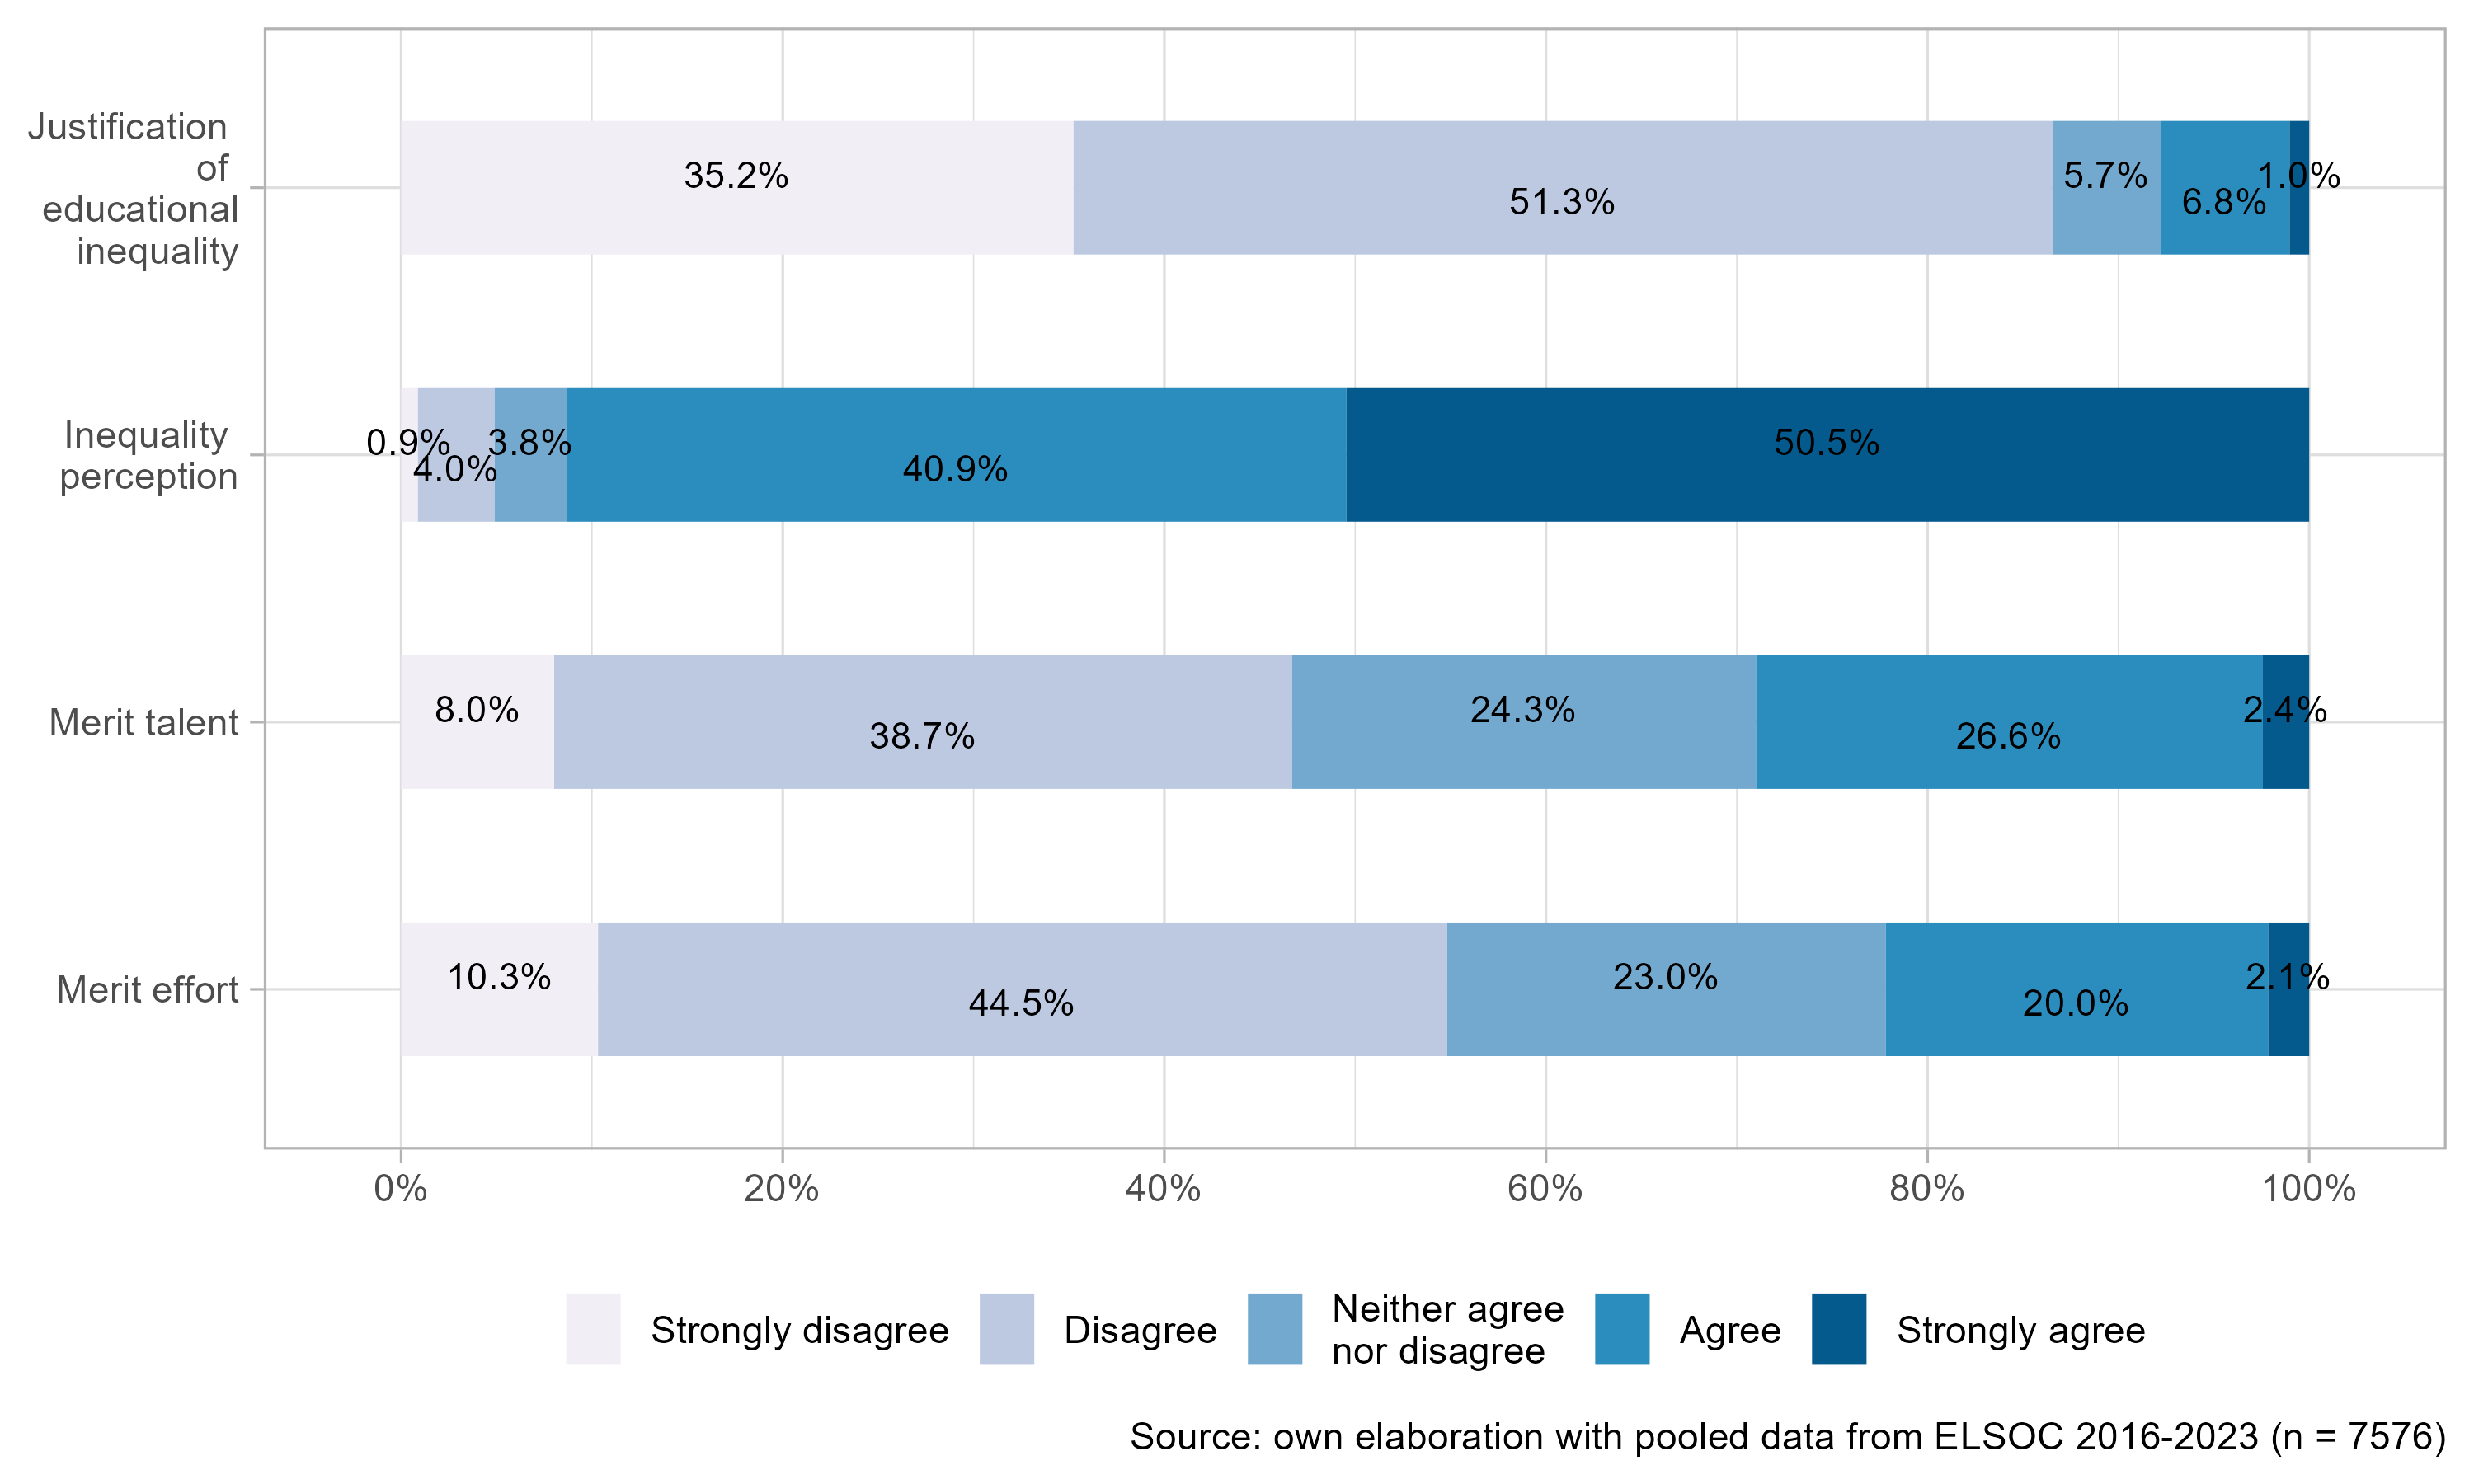
\includegraphics[width=0.85\textwidth,height=\textheight]{output/graphs/merit_plot.png}

}

\caption{\label{fig-frecuencies}Frequency of responses for justification
of educational inequality, perception of inequality, and perception of
meritocracy for all the years analyzed}

\end{figure}%

A third group of variables is included in the analysis to assess the
effect of elements related to the pandemic context. These variables were
only included in the 2021 wave, so each individual's responses were
replicated for the remaining years. The first variable addresses the
belief regarding whether, in the context of the pandemic, it is more
important to give priority to economic activity than to the health of
the population, measured on a Likert scale from (1) ``strongly
disagree'' to (2) ``strongly agree''. The second variable is a dummy
(No/Yes) that captures whether individuals received state benefits
during the pandemic (e.g., Food Box, Emergency Family Income,
Contribution for the Middle Class, or others).

For testing the hypothesis regarding status we considered educational
level and household income. Also, we included subjective social status
as it has been argued that perceived social status is a relevant
predictor of attitudes toward economic inequality (Schneider and
Castillo 2015; Castillo et al. 2019). In addition, such subjective
measures can complement objective measures in predicting life chances
(Oesch and Vigna 2023), which are arguably connected to how individuals
experience economic inequality. In this regard, it has been argued that
how people form their views on their standing in society results from
experiences with direct socioeconomic circumstances and social
comparison processes with reference groups (Condon and Wichowsky 2020).
Finally, political identification on a left-right scale, age groups, and
gender were included as control variables. Table~\ref{tbl-descriptives}
shows the whole set of independent variables, the corresponding items,
response categories, and frequencies.

\begin{longtable}[]{@{}l@{}}
\caption{Independent variables}\label{tbl-descriptives}\tabularnewline
\toprule\noalign{}
\endfirsthead
\endhead
\bottomrule\noalign{}
\endlastfoot
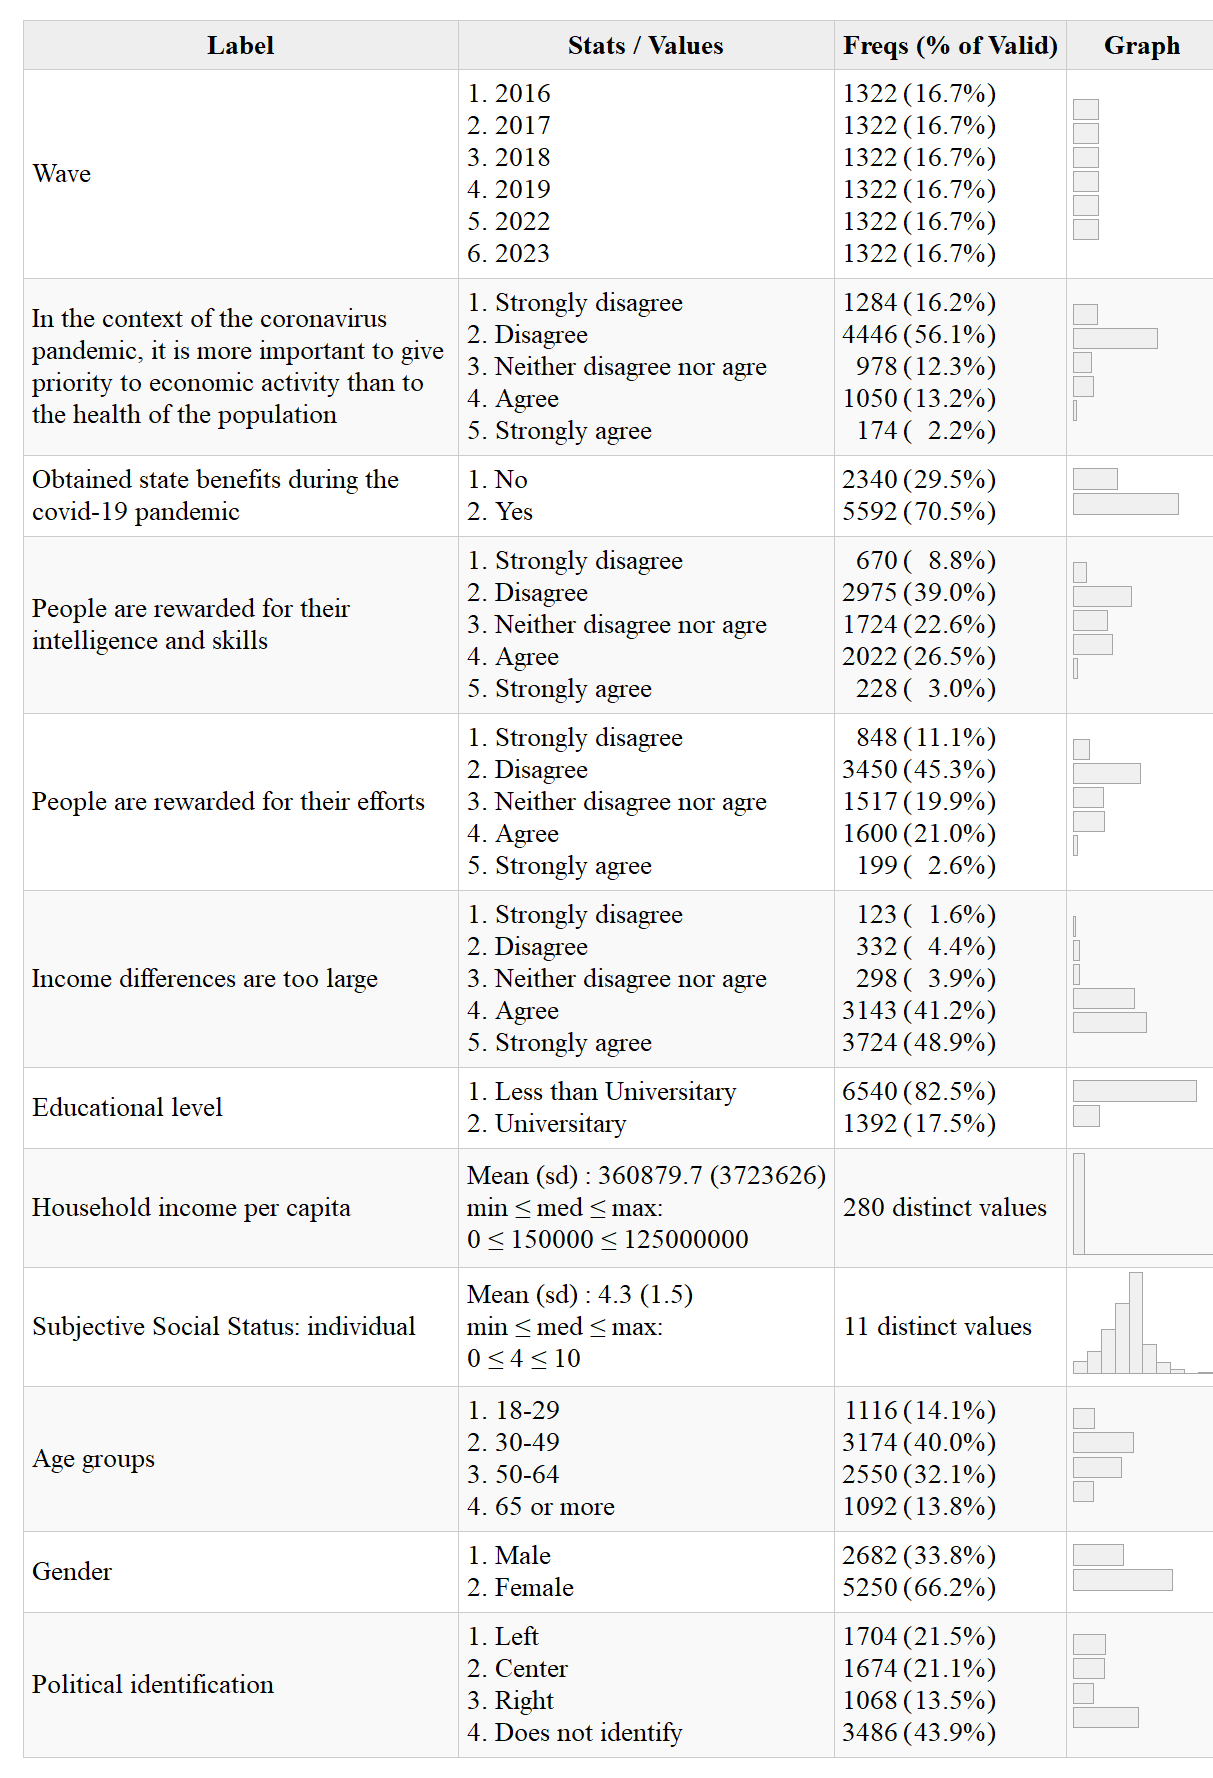
\includegraphics{output/tables/desc02.png} \\
\end{longtable}

\subsection{Methods}\label{methods}

Given the hierarchical structure of the data (observations nested in
survey waves), we estimated a series of longitudinal multilevel models
(Singer and Willett 2009). Such an approach is suited to account for the
shared variance among units (in this case individuals), adjusting the
estimation of the standard errors. The linear multilevel models are
estimated using the R library ``lme4'' (Singer and Willett 2009, 4).

\section{Results}\label{results}

Beginning with a descriptive analysis of changes in the justification of
educational inequality between 2016 and 2023, Figure~\ref{fig-alluvial}
illustrates yearly frequencies and transitions between years. Each year
represents stacked porcentual frequencies, whereas the flows in between
reflect the within-subject change of opinions from one year to the next
(Rosvall and Bergstrom 2010). For instance, of the 32.9\% who strongly
disagreed with inequality justification in 2016, about half of them kept
responding the same in 2017, whereas the other half shifted their
opinion to other response categories. In general, the large majority -
between 80 and 90\% - disagrees with the justification of educational
inequality throughout the years. Despite this overall tendency, we also
observe that the disagreement with inequality justification (disagree +
strongly disagree) tends to go down in the last waves. This change is
mostly a result of the increase in the ``agree'' category, which doubles
compared to previous years (from 5.4\% in 2016 to 11\% in 2023).

\begin{figure}[H]

\centering{

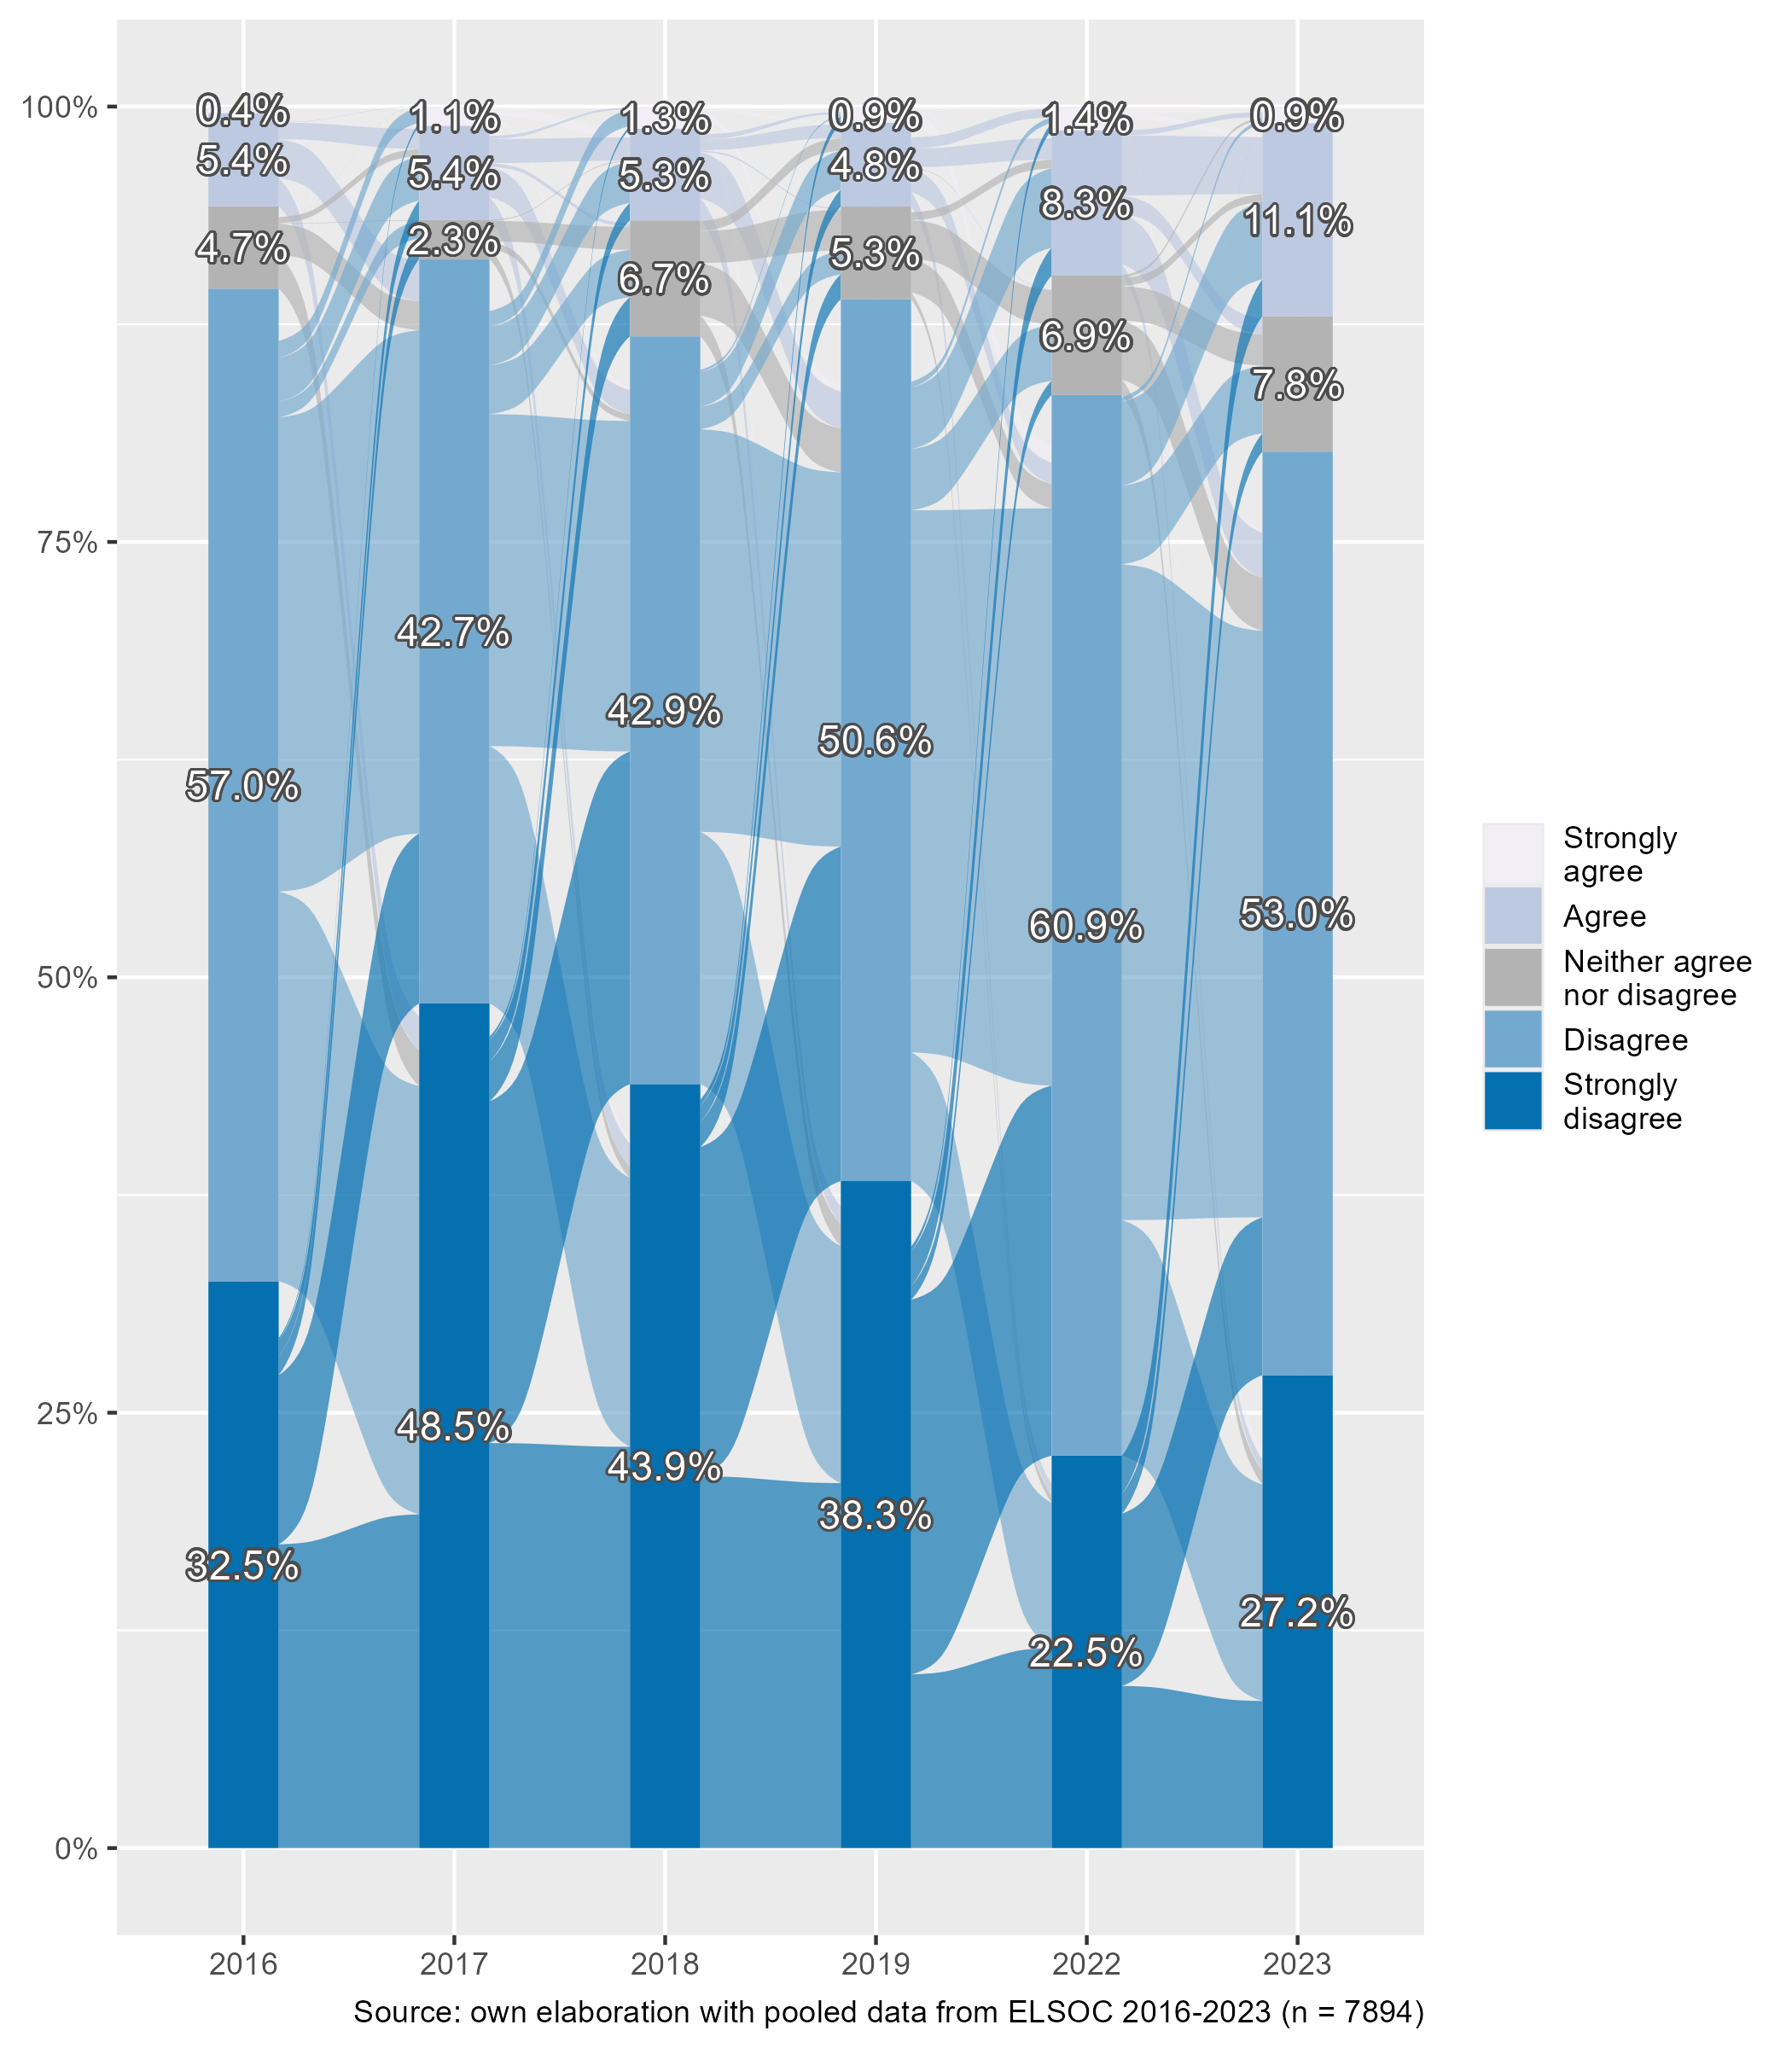
\includegraphics[width=0.85\textwidth,height=\textheight]{output/graphs/alluvial_dep.png}

}

\caption{\label{fig-alluvial}Change in the justification of educational
inequality over time (2016-2023)}

\end{figure}%

Figure~\ref{fig-means} shows the average changes in the main variables
considered for this study. Here we observe that the justification of
educational inequality has the lowest average throughout the years when
compared with the other (independent) variables, whereas the highest
average is consistently represented by inequality perception.
Interestingly, in the last waves of the study (2022-2023) the
justification of inequality increases whereas the perception of
inequality decreases. As the merit variables are concerned, they show a
very similar pattern in terms of averages and changes over the years,
being the perception of meritocracy related to effort always lower than
the one associated with talent.

\begin{figure}[H]

\centering{

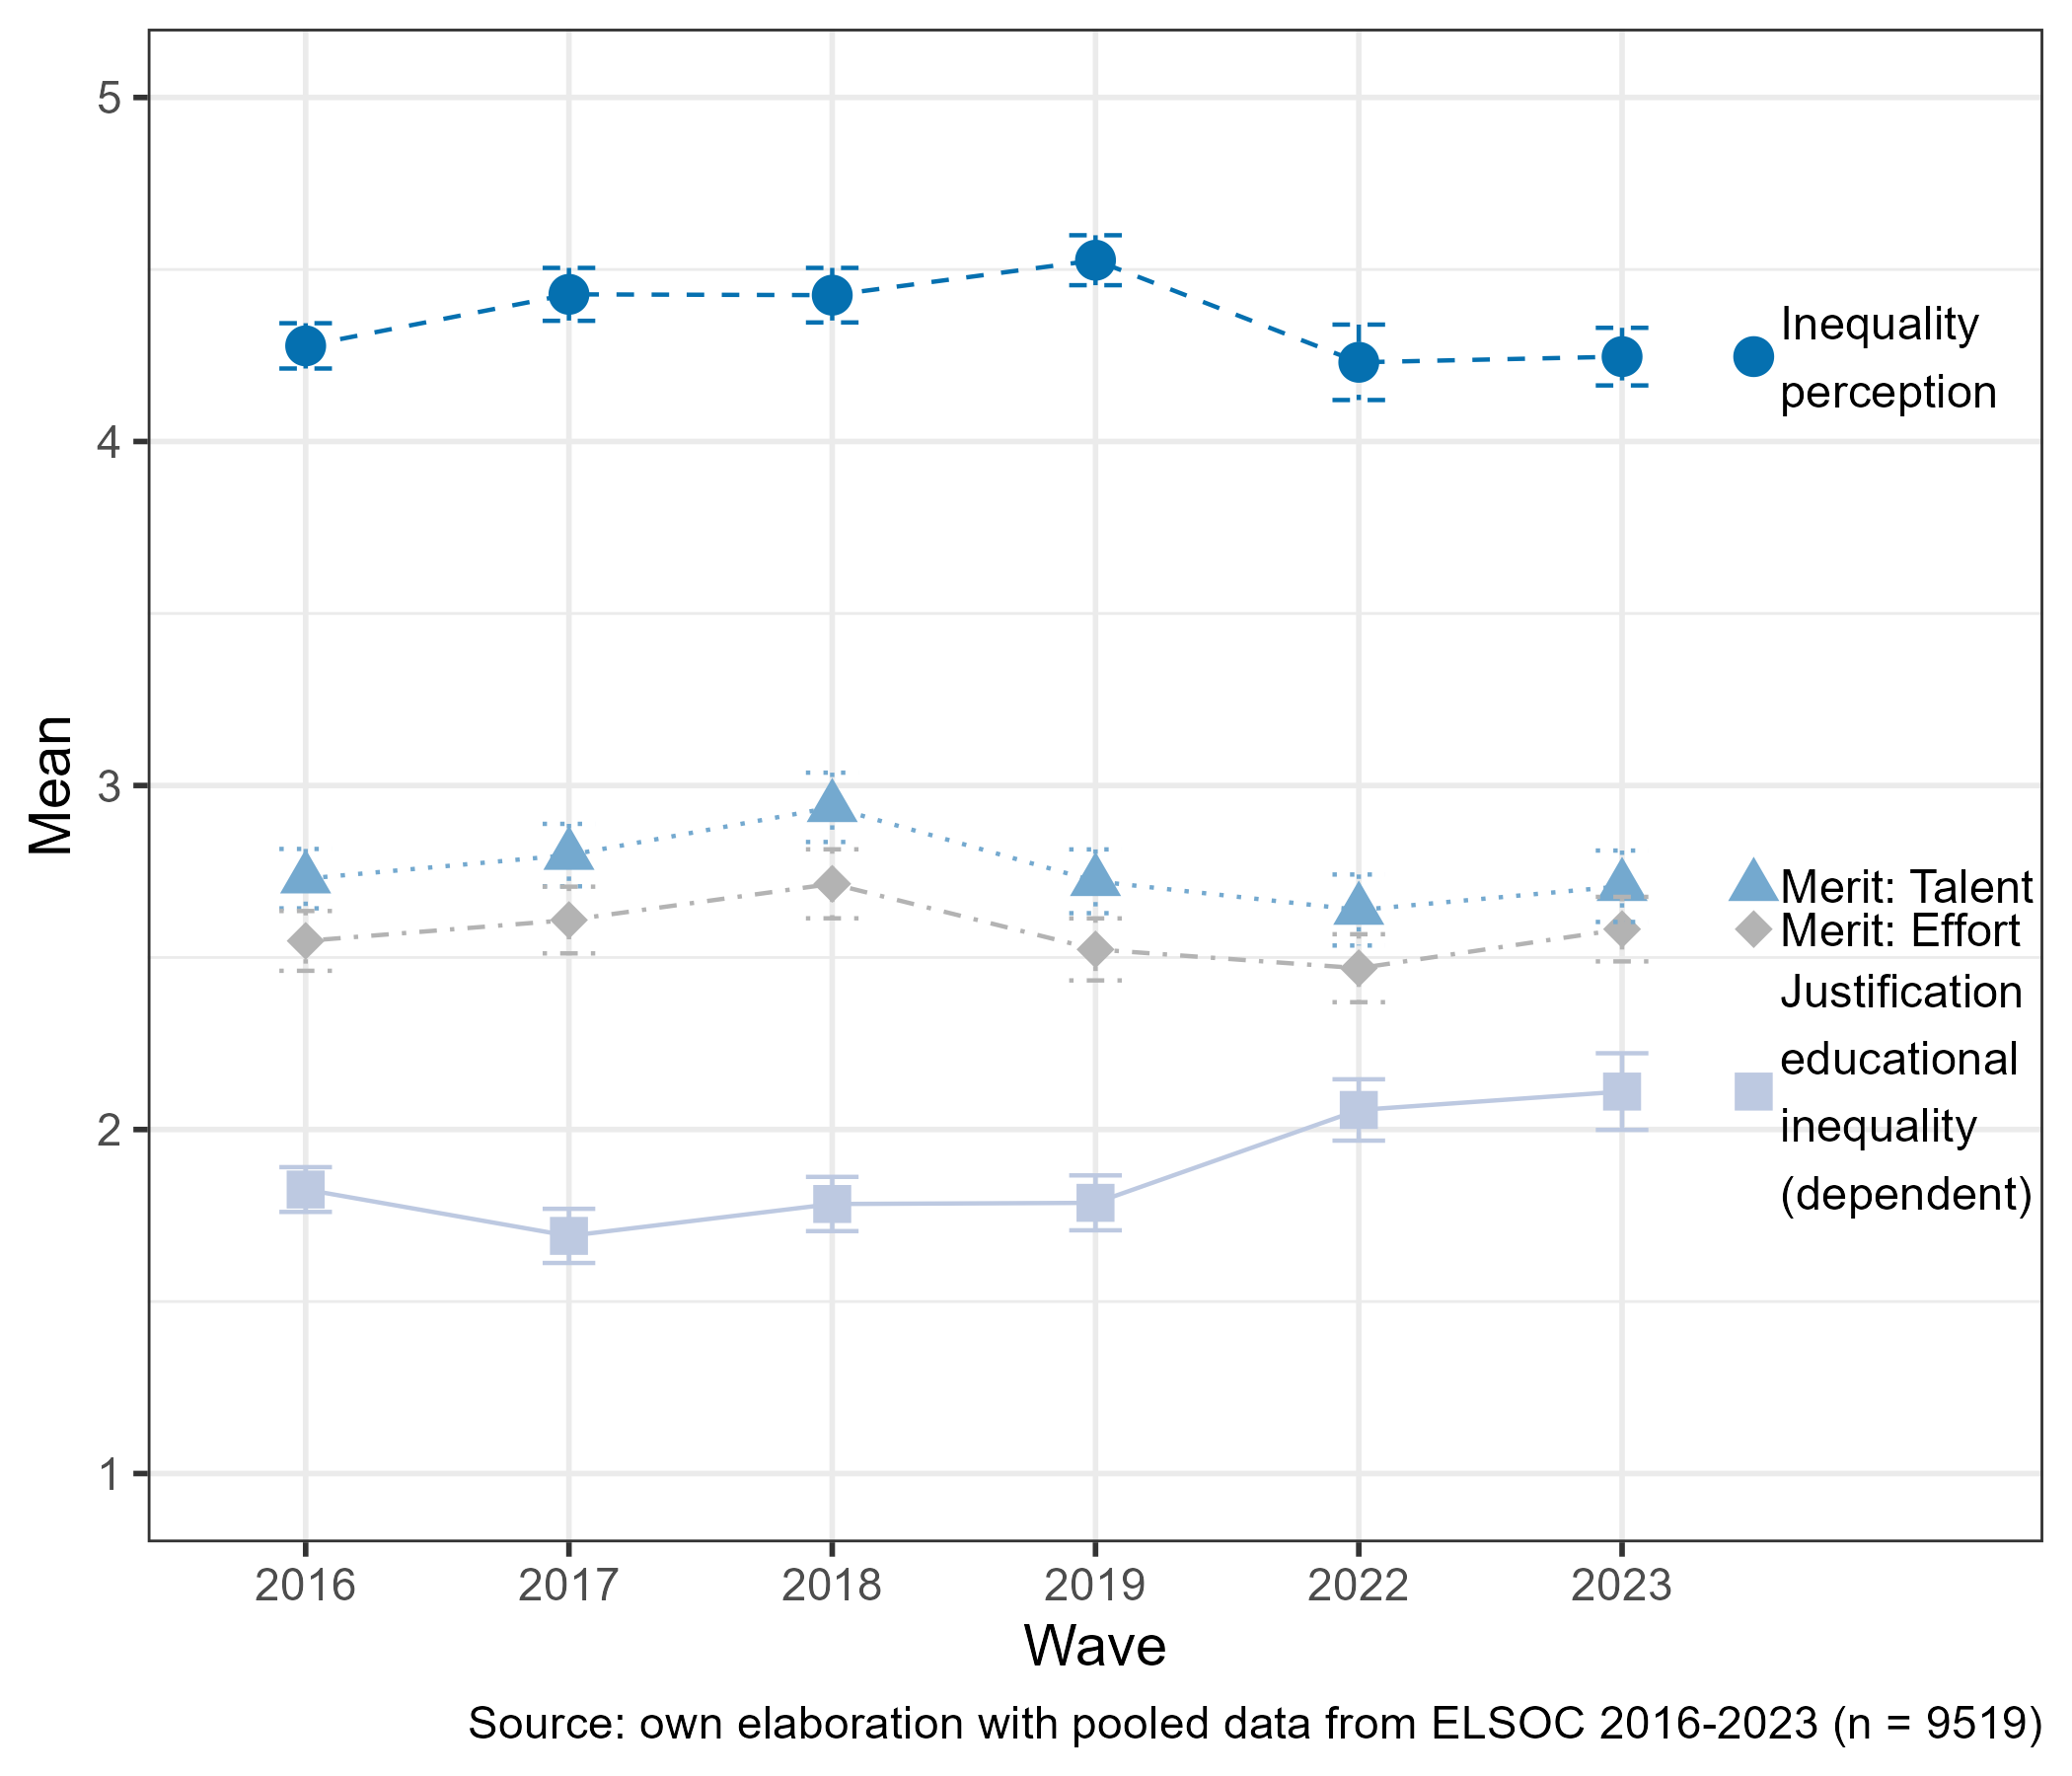
\includegraphics[width=0.85\textwidth,height=\textheight]{output/graphs/years_plot.png}

}

\caption{\label{fig-means}Change in the mean of justification of
educational inequality, perception of inequality, and perception of
meritocracy over the years}

\end{figure}%

Figure~\ref{fig-correlation} presents a correlation matrix of the main
variables analyzed, using data from the last wave (2023). In this
matrix, the correlations vary between low and moderate values. The
correlations between justification of educational inequality with the
two COVID variables are positive, but low. In addition, justification of
education inequality depicts a moderate and negative association with
the perception of inequality (\emph{r}=-0.28, p\textless.01) and a
moderate and positive association with both meritocracy perception
variables (\emph{r}=0.17, p\textless.01; \emph{r}=0.17, p\textless.01).
Regarding the perception of inequality, it presents a moderate and
negative association with both meritocracy perception variables
(\emph{r}=-0.19, p\textless.01; \emph{r}=-0.14, p\textless.01). Finally,
the two meritocracy variables present a high and positive association
with each other (\emph{r}=0.79, p\textless.01).

\begin{figure}[H]

\centering{

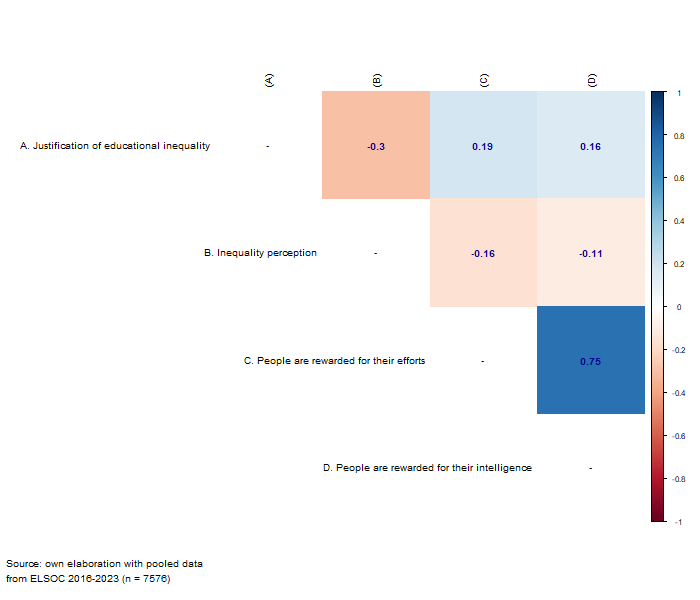
\includegraphics[width=0.85\textwidth,height=\textheight]{output/graphs/corr.png}

}

\caption{\label{fig-correlation}Correlation matrix of the main variables
for the first wave (2016)}

\end{figure}%

\emph{Multilevel models}

Table~\ref{tbl-multilevel} shows the multilevel estimation results for
the justification of educational inequality. Model 1 includes the survey
waves to estimate intertemporal changes in the dependent variable.
Taking 2016 as a reference point, we can observe a staggered decrease in
2017 (\(\beta\)=-0.167, p\textless.001), 2018 (\(\beta\)=-0.059,
p\textless.05), and 2019 (\(\beta\)=-0.03, p\textgreater.05).
Nevertheless, in the last waves of 2022 and 2023 there is a clear
increase in level of justification of educational inequality
(\(\beta\)=0.204, p\textless.001 and \(\beta\)=0.233, p\textless.001),
suggesting a non-linear change in this variable. Attempting to model
this path of change over time, Model 2 incorporates time (survey waves)
as a continuous variable as well as its quadratic term, representing the
nonlinear association initially observed in Model 1. On the one hand,
the survey wave depicts a negative association, expressing an average
decrease in inequality justification over time. On the other hand, the
quadratic wave term is positive, indicating the reversion of this path
in the last measurement points.

Models 3 and 4 adds the two variables about the pandemic context, where
we can see that those who received state benefits during this period
justify less inequality in education compared to those who did not
receive them. Although the effect size is small, it remains significant
when controlling for the rest of the variables in model 8
(\(\beta\)=-0.093, p\textless.01). On the other hand, those who believe
that in this context the economy is more important than the health of
the population justify more inequality in education(\(\beta\)=0.038,
p\textless.05, Model 8).

Models 5 and 6 introduce the meritocratic variables: talent (if
intelligence and abilities are rewarded in society) and effort (if
efforts are rewarded in society). In line with our hypotheses, the
perception that talent is rewarded has a positive influence on the
justification of educational inequality in Model 5 (\(\beta\)=0.055,
p\textless.001). However, when controlling for the perception that
effort is rewarded, this effect is no longer significant. In this sense,
Model 6 shows that the perception that effort is rewarded in society is
not only positively associated with the justification of educational
inequality (\(\beta\)=0.083, p\textless.001), but it has a larger weight
than the perception of talent. Regarding inequality perception (added in
Model 7), it depicts a negative association with the justification of
educational inequality, remaining stable when controlling for the rest
of the variables.

Model 8 adds the socioeconomic variables to test hypothesis 7. Although
educational level and household per capita income are not significant in
this model, controlling for all variables in the next models, household
per capita income depicts a positive effect (\(\beta\)=0.001,
p\textless.05). The inclusion of other controls as being right-wing
(compared to being left-wing) shows a positive association with
justification of educational inequality (\(\beta\)=0.27,
p\textless.001), whereas being a women (compared to men) had a negative
effect (\(\beta\)=-0.08, p\textless.001). Subjective social status and
age had no significant effect when controlling for all the variables
analyzed. The full model specification can be seen in the appendix (see
Table~\ref{tbl-multilevel-full}).

\begin{table}

\caption{\label{tbl-multilevel}Multilevel longitudinal models for the
justification of inequality in education}

\centering{

~

Model 1

Model 2

Model 3

Model 4

Model 5

Model 6

Model 7

Model 8

Intercept

1.847***

1.853***

1.920***

1.776***

1.641***

1.563***

2.174***

2.183***

~

(0.026)

(0.038)

(0.048)

(0.064)

(0.068)

(0.069)

(0.086)

(0.120)

Wave (Ref.= Wave 2016)

~

~

~

~

~

~

~

~

~

~

~

~

~

~

~

~

~

~~~~~Wave 2017

-0.167***

~

~

~

~

~

~

~

~

(0.029)

~

~

~

~

~

~

~

~~~~~Wave 2018

-0.059*

~

~

~

~

~

~

~

~

(0.029)

~

~

~

~

~

~

~

~~~~~Wave 2019

-0.030

~

~

~

~

~

~

~

~

(0.029)

~

~

~

~

~

~

~

~~~~~Wave 2022

0.204***

~

~

~

~

~

~

~

~

(0.030)

~

~

~

~

~

~

~

~~~~~Wave 2023

0.233***

~

~

~

~

~

~

~

~

(0.029)

~

~

~

~

~

~

~

Wave

~

-0.073***

-0.073***

-0.073***

-0.076***

-0.076***

-0.052**

-0.052**

~

~

(0.020)

(0.020)

(0.020)

(0.020)

(0.020)

(0.020)

(0.020)

Wave\^{}2

~

0.016***

0.016***

0.016***

0.016***

0.016***

0.013***

0.013***

~

~

(0.002)

(0.002)

(0.002)

(0.002)

(0.002)

(0.002)

(0.002)

Covid: receive state benefits

~

~

-0.095*

-0.097*

-0.100*

-0.102*

-0.102**

-0.093*

~

~

~

(0.041)

(0.041)

(0.040)

(0.040)

(0.039)

(0.041)

Covid: economy more important than health

~

~

~

0.065***

0.060**

0.055**

0.049**

0.038*

~

~

~

~

(0.019)

(0.019)

(0.019)

(0.019)

(0.019)

Merit: Talent

~

~

~

~

0.055***

-0.002

-0.003

-0.005

~

~

~

~

~

(0.010)

(0.012)

(0.012)

(0.012)

Merit: Effort

~

~

~

~

~

0.096***

0.084***

0.083***

~

~

~

~

~

~

(0.013)

(0.013)

(0.013)

Inequality perception

~

~

~

~

~

~

-0.135***

-0.134***

~

~

~

~

~

~

~

(0.012)

(0.012)

Universitary (Ref.= Less than universitary)

~

~

~

~

~

~

~

-0.048

~

~

~

~

~

~

~

~

(0.046)

Household income

~

~

~

~

~

~

~

0.001*

~

~

~

~

~

~

~

~

(0.000)

Controls

No

No

No

No

No

No

No

Yes

BIC

29667.072

29670.297

29678.484

29682.436

29668.980

29626.960

29510.881

29626.312

Num. obs.

7576

7576

7576

7576

7576

7576

7576

7576

Num. groups: Individuals

1322

1322

1322

1322

1322

1322

1322

1322

Var: Individuals (Intercept)

0.185

0.184

0.183

0.179

0.174

0.170

0.164

0.159

Var: Residual

0.497

0.500

0.500

0.500

0.499

0.496

0.488

0.488

*** p \textless{} 0.001; ** p \textless{} 0.01; * p \textless{} 0.05.
Note: Model 8 is controlled by age, gender, political position, and
subjective social status.

}

\end{table}%

In this last part of the analysis we test hypotheses about the effect of
COVID-19 on changes in the relationship between meritocracy and
justification of educational inequality. In hypothesis 5, we proposed
that the association between the perception of meritocracy and
justification of inequality is mitigated in times of crisis, as
meritocratic ideals might have been weakened due to critical situations
associated with the COVID-19 pandemic. We test this hypothesis through
interaction effects, shown in Table~\ref{tbl-interact}. The first model
is shown as the baseline model. It is the same as model 8 in
Table~\ref{tbl-multilevel}, but only shows the variables involved in the
interaction for the sake of space (all other variables are included).
Model 9 adds the interaction between the perception of talent-based
meritocracy and whether state benefits were received during the
pandemic, whereas Model 10 considers the perception of effort-related
meritocracy for the interaction. Both variables show a negative
significant interaction with receiving state benefits
(\(\beta_{talent}\)=-0.07, p\textless.01; \(\beta_{effort}\)=-0.05,
p\textless.05), meaning that for those who received state benefits the
association between the the justification of inequality and the
perception of effort-based meritocracy lower by 0.05 points, and by 0.07
points regarding the perception of talent-based meritocracy. This last
interaction is depicted in Figure~\ref{fig-interact-talent}, showing
that the positive association between the perception of talent-based
meritocracy and the justification of educational inequality is smaller
for those who received state benefits during the pandemic.

\begin{table}

\caption{\label{tbl-interact}Interaction effects for the justification
of economic inequality}

\centering{

~

Model 8

Model 9

Model 10

Intercept

2.18***

2.03***

2.09***

~

(0.12)

(0.13)

(0.13)

Wave

-0.05**

-0.05*

-0.05**

~

(0.02)

(0.02)

(0.02)

Wave\^{}2

0.01***

0.01***

0.01***

~

(0.00)

(0.00)

(0.00)

Covid: receive state benefits

-0.09*

0.11

0.03

~

(0.04)

(0.07)

(0.07)

Merit: Talent

-0.00

0.05*

-0.01

~

(0.01)

(0.02)

(0.01)

Merit: Effort

0.08***

0.08***

0.12***

~

(0.01)

(0.01)

(0.02)

Receive state benefits * Merit: Talent

~

-0.07**

~

~

~

(0.02)

~

Receive state benefits * Merit: Effort

~

~

-0.05*

~

~

~

(0.02)

BIC

29626.31

29630.35

29636.59

Num. obs.

7576

7576

7576

Num. groups: Individuals

1322

1322

1322

Var: Individuals (Intercept)

0.16

0.16

0.16

Var: Residual

0.49

0.49

0.49

\item *

** p \textless{} 0.001; ** p \textless{} 0.01; * p \textless{} 0.05.
Note: All the models are controlled by educational level, income
quintile, subjective social status, age, gender, political position, and
inequality perception

}

\end{table}%

\begin{figure}[H]

\centering{

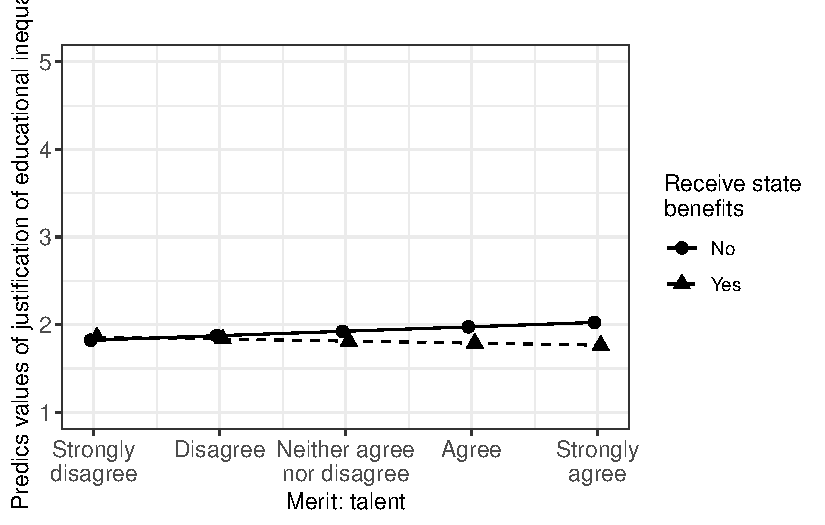
\includegraphics[width=0.85\textwidth,height=\textheight]{paper_files/figure-pdf/fig-interact-talent-1.pdf}

}

\caption{\label{fig-interact-talent}Interaction effect of merit based on
talent and receive state benefits on justification of educational
inequality}

\end{figure}%

\section{Discussion and conclusions}\label{discussion-and-conclusions}

Our research sought to examine the justification of inequality in
education from a longitudinal perspective amid the health crisis
generated by the COVID-19 pandemic. In general, our results showed mixed
evidence about our hypotheses. We argued that in times of crisis,
greater exposure to risk due to the health context would result in a
lower justification of inequality by citizens. In this regard,
longitudinal models showed that the justification of inequality in
education is far from being linear, and whereas a decreasing pattern was
found between 2017 and 2019, there is a striking increase in the
post-pandemic measurement points. Besides, our findings revealed that
those who received benefits justified educational inequality less than
those who did not. Still, given our data limitations it is not possible
to attribute such changes only to the pandemic and the related economic
and social crises. As during this very same period in Chile there were
two (failed) constitutional processes, disentangling different forces
driving public opinion becomes cumbersome and deserves further
qualitative and quantitative studies. Along this line, some recent
studies have argued that the election of a far left-wing constitutional
assembly in the first process generated a backslash effect, mainly due
to several scandals that led to the delegitimation of this assembly.
This could have driven preferences in a conservative direction, which
was reflected in the election of a right-wing second assembly after the
failed first constitutional process (Palanza and Sotomayor 2023; Sazo
2023).

The main focus of this study was on the relationship between meritocracy
and justification of inequality, arguing that those who perceive that
the society in which they live complies with meritocratic principles,
would be more inclined to justify inequality in education. At first
look, the results are consistent with the hypothesis; however, some
nuances are worth attending as the effort dimension prevails over the
talent dimension. In other words, the perception of meritocracy in terms
of rewarded effort is more relevant in justifying access to education
than the perception of talent. This could be explained as that talent
could be more associated with luck in terms of random assignment, and in
this terms would not be enough reason (as it is effort) to justify
educational inequality. Furthermore, we observed that the connection
between perceived meritocracy and the justification of educational
inequality weakened for those who received state benefits, which aligns
with our expectations given the social context in the post-COVID era.
One possible interpretation is that, during times of increased risk,
people may become more skeptical of narratives emphasizing individual
effort over collective efforts. This shift in perspective might also
foster stronger solidarity to protect individual and societal wellbeing.
However, further studies are necessary to explore this phenomenon using
more specific conceptual and methodological approaches.

Regarding the status position, our central hypothesis was that
individuals in more advantaged situations and with greater resources
would tend to defend their interests and justify greater education
inequality. In this regard, our results show a positive relationship
between income and the justification of inequality, which would align
with our argument that rational interests of the better-off that would
lead to a larger inequality justification. Besides status, we also
considered inequality perception, as the literature on attitudes toward
inequality has argued that a greater justification of inequality is
associated with its perceived magnitude. Consistent with this
hypothesis, our results showed that, throughout the years, a larger
perceived economic inequality motivates a lower justification of
inequality in education.

Among the limitations of our study, we can mention at least three.
First, the operationalization of justification of educational inequality
is rather limited. We counted only on a single item for this in this
study, and further work is needed in order to assess the validity and
reliability of measuring such construct. Second, as it has been
established by recent research (Castillo et al. 2023), the perception of
meritocracy can be understood through individual attributions regarding
effort and talent, but also taking into account the role of structural
aspects such as family status and social capital. Due to data
limitations such dimensions were not included here, therefore providing
a partial perspective on the areas of perceived meritocracy. Finally,
there are limitations involving the longitudinal dimension of the data
used. Given constraints for data collection during the pandemic, the
ELSOC study had to shorten the questionnaire in 2021 and unfortunately,
the educational justice indicator was excluded from that survey.
Consequently, the results of temporal change have to be considered
carefully, and further data waves could give us more information on this
matter.

Regarding future studies, the capabilities of the ELSOC longitudinal
database are not limited to micro-level estimates. In this regard,
thanks to the sampling strategy of the survey, it would be possible to
make contextual estimates at the municipality level. For instance,
statistical models could include contextual information from
administrative data sources, allowing testing for hypotheses that
include contextual socioeconomic inequality as well as its dynamics over
time. Furthermore, this dataset could be used for comparing inequality
justification in policy areas besides education, such as health and
pensions. Future studies may shed light on how meritocratic perceptions
and beliefs affect differently such areas and their changes over time,
which would give relevant hints from social sciences for the discussion
about societal and cultural changes as well as their impacts on
solidarity and social cohesion.

\section{References}\label{references}

\phantomsection\label{refs}
\begin{CSLReferences}{1}{0}
\bibitem[\citeproctext]{ref-barry_theories_1989}
Barry, Brian. 1989. \emph{Theories of Justice}. A Treatise on Social
Justice 1. Berkeley: Univ. of California Pr.

\bibitem[\citeproctext]{ref-batruch_belief_2023}
Batruch, Anatolia, Jolanda Jetten, Herman Van De Werfhorst, Céline
Darnon, and Fabrizio Butera. 2023. {``Belief in {School Meritocracy} and
the {Legitimization} of {Social} and {Income Inequality}.''}
\emph{Social Psychological and Personality Science} 14 (5): 621--35.
\url{https://doi.org/10.1177/19485506221111017}.

\bibitem[\citeproctext]{ref-bell_politics_2020}
Bell, Elizabeth. 2020. {``The {Politics} of {Designing Tuition-Free
College}: {How Socially Constructed Target Populations Influence Policy
Support}.''} \emph{The Journal of Higher Education} 91 (6): 888--926.
\url{https://doi.org/10.1080/00221546.2019.1706015}.

\bibitem[\citeproctext]{ref-bellei_estudio_2013}
Bellei, Cristián. 2013. {``El Estudio de La Segregaci{ó}n
Socioecon{ó}mica y Acad{é}mica de La Educaci{ó}n Chilena.''}
\emph{Estudios Pedag{ó}gicos (Valdivia)} 39 (1): 325--45.
\url{https://doi.org/10.4067/S0718-07052013000100019}.

\bibitem[\citeproctext]{ref-breznau_welfare_2021}
Breznau, Nate. 2021. {``The Welfare State and Risk Perceptions: The
{Novel Coronavirus Pandemic} and Public Concern in 70 Countries.''}
\emph{European Societies} 23 (sup1): S33--46.
\url{https://doi.org/10.1080/14616696.2020.1793215}.

\bibitem[\citeproctext]{ref-busemeyer_welfare_2020}
Busemeyer, Marius R., and Torben Iversen. 2020. {``The {Welfare State}
with {Private Alternatives}: {The Transformation} of {Popular Support}
for {Social Insurance}.''} \emph{The Journal of Politics} 82 (2):
671--86. \url{https://doi.org/10.1086/706980}.

\bibitem[\citeproctext]{ref-castillo_perception_2022}
Castillo, Juan Carlos, Juan-Diego García-Castro, and Martín Venegas.
2022. {``Perception of Economic Inequality: Concepts, Associated Factors
and Prospects of a Burgeoning Research Agenda.''} \emph{International
Journal of Social Psychology} 37 (1): 180--207.
\url{https://doi.org/10.1080/02134748.2021.2009275}.

\bibitem[\citeproctext]{ref-castillo_multidimensional_2023}
Castillo, Juan Carlos, Julio Iturra, Luis Maldonado, Jorge Atria, and
Francisco Meneses. 2023. {``A {Multidimensional Approach} for {Measuring
Meritocratic Beliefs}: {Advantages}, {Limitations} and {Alternatives} to
the {ISSP Social Inequality Survey}.''} \emph{International Journal of
Sociology}, October, 1--25.
\url{https://doi.org/10.1080/00207659.2023.2274712}.

\bibitem[\citeproctext]{ref-castillo_clivajes_2013}
Castillo, Juan Carlos, Ignacio Madero-Cabib, and Alan Salamovich. 2013.
{``Clivajes {Partidarios} y {Cambios} En Las {Preferencias
Redistributivas} En {Chile}.''} \emph{Revista de Ciencia Pol{í}tica
(Santiago)} 33 (2): 469--88.
\url{https://doi.org/10.4067/S0718-090X2013000200003}.

\bibitem[\citeproctext]{ref-castillo_percepcion_2019}
Castillo, Juan Carlos, Daniel Miranda, and Diego Carrasco. 2012.
{``Percepci{ó}n de {Desigualdad Econ{ó}mica} En {Chile}: {Medici{ó}n},
{Diferencias} y {Determinantes}.''} \emph{Psykhe (Santiago)} 21 (1):
99--114. \url{https://doi.org/10.4067/S0718-22282012000100007}.

\bibitem[\citeproctext]{ref-castillo_meritocracia_2019}
Castillo, Juan Carlos, Alex Torres, Jorge Atria, and Luis Maldonado.
2019. {``Meritocracia y Desigualdad Econ{ó}mica: {Percepciones},
Preferencias e Implicancias.''} \emph{Revista Internacional de
Sociolog{í}a} 77 (1): 117.
\url{https://doi.org/10.3989/ris.2019.77.1.17.114}.

\bibitem[\citeproctext]{ref-coes_radiografia_2023}
COES. 2023. {``Radiograf{í}a Del {Cambio Social}: {An{á}lisis} de
{Resultados Longitudinales ELSOC} 2016-2021.''} Santiago de Chile,
Chile: Centro de Estudios de Conflicto y Cohesi{ó}n Social.

\bibitem[\citeproctext]{ref-condon_inequality_2020}
Condon, Meghan, and Amber Wichowsky. 2020. {``Inequality in the {Social
Mind}: {Social Comparison} and {Support} for {Redistribution}.''}
\emph{The Journal of Politics} 82 (1): 149--61.
\url{https://doi.org/10.1086/705686}.

\bibitem[\citeproctext]{ref-corvalan_mercado_2016}
Corvalán, Javier, Alejandro Carrasco, and J. E. García-Huidobro, eds.
2016. \emph{Mercado Escolar: {Libertad}, Diversidad y Desigualdad}. 1st
ed. Santiago: Ediciones UC. \url{https://doi.org/10.2307/j.ctv14rmrhn}.

\bibitem[\citeproctext]{ref-darmody_impacts_2021}
Darmody, Merike, Emer Smyth, and Helen Russell. 2021. {``Impacts of the
{COVID-19 Control Measures} on {Widening Educational Inequalities}.''}
\emph{YOUNG} 29 (4): 366--80.
\url{https://doi.org/10.1177/11033088211027412}.

\bibitem[\citeproctext]{ref-day_perceived_2023}
Day, Martin V., and Michael I. Norton. 2023. {``Perceived and {Ideal
Inequality} in {University Endowments} in the {United States}.''}
\emph{Personality and Social Psychology Bulletin} 49 (8): 1151--65.
\url{https://doi.org/10.1177/01461672221083766}.

\bibitem[\citeproctext]{ref-donoso_when_2016}
Donoso, Sofia. 2016. {``When {Social Movements Become} a {Democratizing
Force}: {The Political Impact} of the {Student Movement} in {Chile}.''}
In \emph{Research in {Social Movements}, {Conflicts} and {Change}},
edited by Thomas Davies, Holly Eva Ryan, and Alejandro Milcíades Peña,
39:167--96. Emerald Group Publishing Limited.
\url{https://doi.org/10.1108/S0163-786X20160000039008}.

\bibitem[\citeproctext]{ref-elsoc_estudio_2022}
ELSOC, Survey Team. 2022. {``Estudio {Longitudinal Social} de
{Chile}.''} Harvard Dataverse. \url{https://doi.org/10.7910/dvn/0kirbj}.

\bibitem[\citeproctext]{ref-gimpelson_misperceiving_2018}
Gimpelson, Vladimir, and Daniel Treisman. 2018. {``Misperceiving
Inequality.''} \emph{Economics \& Politics} 30 (1): 27--54.
\url{https://doi.org/10.1111/ecpo.12103}.

\bibitem[\citeproctext]{ref-goldin_meritocracy_2000}
Goldin, Claudia. 2000. {``Meritocracy and {Economic Inequality}.
{Edited} by {Kenneth Arrow}, {Samuel Bowles}, and {Steven Durlauf} (
{Princeton}, {Princeton University Press}, 2000) 348 Pp.''}
\emph{Journal of Interdisciplinary History} 31 (3): 431a--433.
\url{https://doi.org/10.1162/jinh.2000.31.3.431a}.

\bibitem[\citeproctext]{ref-hadjar_meritokratie_2008}
Hadjar, Andreas. 2008. \emph{{Meritokratie als Legitimationsprinzip}}.
Wiesbaden: VS Verlag f{ü}r Sozialwissenschaften.

\bibitem[\citeproctext]{ref-hale_global_2021}
Hale, Thomas, Noam Angrist, Rafael Goldszmidt, Beatriz Kira, Anna
Petherick, Toby Phillips, Samuel Webster, et al. 2021. {``A Global Panel
Database of Pandemic Policies ({Oxford COVID-19 Government Response
Tracker}).''} \emph{Nature Human Behaviour} 5 (4): 529--38.
\url{https://doi.org/10.1038/s41562-021-01079-8}.

\bibitem[\citeproctext]{ref-hankivsky_introduction_2022}
Hankivsky, Olena, Marina Morrow, and Colleen Varcoe. 2022.
{``{INTRODUCTION Women}'s {Health} in {Canada}: {Critical Intersectional
Perspectives} on {Theory} and {Policy}.''} In \emph{Women's {Health} in
{Canada}}, edited by Marina Morrow, Olena Hankivsky, and Colleen Varcoe,
1--10. University of Toronto Press.
\url{https://doi.org/10.3138/9781442623958-003}.

\bibitem[\citeproctext]{ref-igliozzi_fair_2024}
Igliozzi, David, Yael Granot, and Victor Ottati. 2024. {``A Fair Share:
{Effects} of Disparity, Allocation Strategy and System Justification on
Perceptions of Policy Support in the Education Domain.''} \emph{European
Journal of Social Psychology}, February, ejsp.3040.
\url{https://doi.org/10.1002/ejsp.3040}.

\bibitem[\citeproctext]{ref-institutonacionaldeestadisticas_resultados_2022}
Instituto Nacional de Estadísticas. 2022. {``Resultados de La Encuesta
Nacional de Empleo: {Serie} Anualizada (2006 - 2023).''} Instituto
Nacional de Estad{í}sticas.

\bibitem[\citeproctext]{ref-janmaat_subjective_2013}
Janmaat, Jan Germen. 2013. {``Subjective Inequality: {A} Review of
International Comparative Studies on People's Views about Inequality.''}
\emph{Archives Europeennes de Sociologie} 54 (3): 357--89.
\url{https://doi.org/10.1017/S0003975613000209}.

\bibitem[\citeproctext]{ref-joignant_informe_2020}
Joignant, Alfredo, Matías Garretón, Nicolás M. Somma, and Tomás Campos.
2020. {``Informe Anual: {Observatorio} de Conflictos 2020.''} Centro de
Estudios de Conflicto y Cohesi{ó}n Social (COES).

\bibitem[\citeproctext]{ref-joiko_cuasimercado_2019}
Joiko, Sara. 2019. {``{El cuasi-mercado educativo en Chile: desarrollo y
consecuencias}.''} \emph{Revista Electr{ó}nica Di{á}logos Educativos;
Vol. 12 N{ú}m. 23 (2012); 148-174}, April.

\bibitem[\citeproctext]{ref-jost_psychology_2003}
Jost, John, and Orsolya Hunyady. 2003. {``The Psychology of System
Justification and the Palliative Function of Ideology.''} \emph{European
Review of Social Psychology} 13 (1): 111--53.
\url{https://doi.org/10.1080/10463280240000046}.

\bibitem[\citeproctext]{ref-kelley_legitimate_2021}
Kelley, Jonathan, and M. D. R. Evans. 2021. {``Legitimate Earnings
Inequality and National Welfare Commitment: {Correspondence} Between
Economic Institutions and the Pay 80,000+ People in 30 Nations Think
Legitimate for Ordinary Jobs and for Elite Jobs.''} \emph{Social Science
Research} 94 (February): 102446.
\url{https://doi.org/10.1016/j.ssresearch.2020.102446}.

\bibitem[\citeproctext]{ref-lee_fairness_2023}
Lee, Jung-Sook, and Meghan Stacey. 2023. {``Fairness Perceptions of
Educational Inequality: The Effects of Self-Interest and Neoliberal
Orientations.''} \emph{The Australian Educational Researcher}, May.
\url{https://doi.org/10.1007/s13384-023-00636-6}.

\bibitem[\citeproctext]{ref-lindh_public_2015}
Lindh, Arvid. 2015. {``Public {Opinion} Against {Markets}? {Attitudes}
Towards {Market Distribution} of {Social Services} -- {A Comparison} of
17 {Countries}.''} \emph{Social Policy \& Administration} 49 (7):
887--910. \url{https://doi.org/10.1111/spol.12105}.

\bibitem[\citeproctext]{ref-mcnamee_meritocracy_2004}
McNamee, Stephen, and Robert Miller. 2004. \emph{The Meritocracy Myth}.
2004th ed. Lanham Md.: Rowman \& Littlefield.

\bibitem[\citeproctext]{ref-mijs_stratified_2016}
Mijs, Jonathan. 2016. {``Stratified {Failure}: {Educational
Stratification} and {Students}' {Attributions} of {Their Mathematics
Performance} in 24 {Countries}.''} \emph{Sociology of Education} 89 (2):
137--53. \url{https://doi.org/10.1177/0038040716636434}.

\bibitem[\citeproctext]{ref-mijs_visualizing_2018}
---------. 2018. {``Visualizing {Belief} in {Meritocracy},
1930--2010.''} \emph{Socius} 4 (January): 2378023118811805.
\url{https://doi.org/10.1177/2378023118811805}.

\bibitem[\citeproctext]{ref-mijs_paradox_2021}
---------. 2021. {``The Paradox of Inequality: Income Inequality and
Belief in Meritocracy Go Hand in Hand.''} \emph{Socio-Economic Review}
19 (1): 7--35. \url{https://doi.org/10.1093/ser/mwy051}.

\bibitem[\citeproctext]{ref-ministeriodedesarrollosocialyfamilia_resultados_2023}
Ministerio de Desarrollo Social y Familia. 2023. {``Resultados de
{Ingresos} de Los {Hogares CASEN} 2022.''} Ministerio de Desarrollo
Social y Familia, Gobierno de Chile.

\bibitem[\citeproctext]{ref-oecd_pisa_2023}
OECD. 2023. \emph{{PISA} 2022 {Results} ({Volume I}): {The State} of
{Learning} and {Equity} in {Education}}. {PISA}. OECD.
\url{https://doi.org/10.1787/53f23881-en}.

\bibitem[\citeproctext]{ref-oesch_subjective_2023}
Oesch, Daniel, and Nathalie Vigna. 2023. {``Subjective Social Class Has
a Bad Name, but Predicts Life Chances Well.''} \emph{Research in Social
Stratification and Mobility} 83 (February): 100759.
\url{https://doi.org/10.1016/j.rssm.2023.100759}.

\bibitem[\citeproctext]{ref-palanza_chiles_2023}
Palanza, Valeria, and Patricia Sotomayor. 2023. {``Chile's Failed
Constitutional Intent: {Polarization}, Fragmentation, Haste and
Delegitimization.''} \emph{Global Constitutionalism}, September, 1--10.
\url{https://doi.org/10.1017/S204538172300028X}.

\bibitem[\citeproctext]{ref-ramos_educacion_2022}
Ramos, Marcela, ed. 2022. \emph{Educaci{ó}n: {La} Promesa Incumplida:
Esfuerzo, Miedos y Esperanzas de Familias Chilenas En El Mercado
Escolar}. Primera edici{ó}n. Santiago, Chile: Catalonia : CIAE, Centro
de Investigaci{ó}n Avanzada en Educaci{ó}n, Universidad de Chile.

\bibitem[\citeproctext]{ref-reyes-housholder_chile_2019}
Reyes-Housholder, Catherine, and Beatriz Roque. 2019. {``Chile 2018:
Desaf{í}os Al Poder de g{é}nero Desde La Calle Hasta {La Moneda}.''}
\emph{Revista de Ciencia Pol{í}tica (Santiago)} 39 (2): 191--216.
\url{https://doi.org/10.4067/S0718-090X2019000200191}.

\bibitem[\citeproctext]{ref-rosvall_mapping_2010}
Rosvall, Martin, and Carl T. Bergstrom. 2010. {``Mapping {Change} in
{Large Networks}.''} Edited by Fabio Rapallo. \emph{PLoS ONE} 5 (1):
e8694. \url{https://doi.org/10.1371/journal.pone.0008694}.

\bibitem[\citeproctext]{ref-sandel_tyranny_2020}
Sandel, Michael J. 2020. \emph{The Tyranny of Merit: {What}'s Become of
the Common Good?} First edition. New York: {Farrar, Straus and Giroux}.

\bibitem[\citeproctext]{ref-sazo_chile_2023}
Sazo, Diego. 2023. {``Chile 2022: {From} Great Expectations to Rising
Pessimism.''} \emph{Revista de Ciencia Pol{í}tica (Santiago)}, no.
ahead. \url{https://doi.org/10.4067/s0718-090x2023005000118}.

\bibitem[\citeproctext]{ref-schneider_poverty_2015}
Schneider, Simone M, and Juan Carlos Castillo. 2015. {``Poverty
{Attributions} and the {Perceived Justice} of {Income Inequality} : {A
Comparison} of {East} and {West Germany}.''}
\url{https://doi.org/10.1177/0190272515589298}.

\bibitem[\citeproctext]{ref-singer_applied_2009}
Singer, Judith D., and John B. Willett. 2009. \emph{Applied Longitudinal
Data Analysis: Modeling Change and Event Occurence}. New York: Oxford
University Press, Incorporated.

\bibitem[\citeproctext]{ref-somma_no_2021}
Somma, Nicolás M., Matías Bargsted, Rodolfo Disi Pavlic, and Rodrigo M.
Medel. 2021. {``No Water in the Oasis: The {Chilean Spring} of
2019--2020.''} \emph{Social Movement Studies} 20 (4): 495--502.
\url{https://doi.org/10.1080/14742837.2020.1727737}.

\bibitem[\citeproctext]{ref-sonhing_merit_2011}
Son Hing, Leanne S., D. Ramona, Mark P. Zanna, Donna M. Garcia,
Stephanie S. Gee, and Katie Orazietti. 2011. {``The Merit of
Meritocracy.''} \emph{Journal of Personality and Social Psychology} 101
(3): 433--50. \url{https://doi.org/10.1037/a0024618}.

\bibitem[\citeproctext]{ref-sonhing_failure_2019}
Son Hing, Leanne S., Anne E. Wilson, Peter Gourevitch, Jaslyn English,
and Parco Sin. 2019. {``Failure to {Respond} to {Rising Income
Inequality}: {Processes That Legitimize Growing Disparities}.''}
\emph{Daedalus} 148 (3): 105--35.
\url{https://doi.org/10.1162/daed_a_01752}.

\bibitem[\citeproctext]{ref-trump_income_2018}
Trump, Kris-Stella. 2018. {``Income {Inequality Influences Perceptions}
of {Legitimate Income Differences}.''} \emph{British Journal of
Political Science} 48 (4): 929--52.
\url{https://doi.org/10.1017/S0007123416000326}.

\bibitem[\citeproctext]{ref-valant_politics_2016}
Valant, Jon, and Daniel A. Newark. 2016. {``The {Politics} of
{Achievement Gaps}: {U}.{S}. {Public Opinion} on {Race-Based} and
{Wealth-Based Differences} in {Test Scores}.''} \emph{Educational
Researcher} 45 (6): 331--46.
\url{https://doi.org/10.3102/0013189X16658447}.

\bibitem[\citeproctext]{ref-young_rise_1962}
Young, M. 1962. \emph{The Rise of the Meritocracy}. Baltimore: Penguin
Books.

\end{CSLReferences}

\section*{(APPENDIX) Appendix}\label{appendix-appendix}
\addcontentsline{toc}{section}{(APPENDIX) Appendix}

\appendix \section{Appendix}

\begin{table}

\caption{\label{tbl-multilevel-full}Complete multilevel longitudinal
models for the justification of inequality in education}

\centering{

~

Model 1

Model 2

Model 3

Model 4

Model 5

Model 6

Model 7

Intercept

1.847***

1.853***

1.873***

1.741***

1.664***

2.276***

2.277***

~

(0.026)

(0.038)

(0.090)

(0.092)

(0.092)

(0.105)

(0.138)

Wave (Ref.= Wave 2016)

~

~

~

~

~

~

~

~

~

~

~

~

~

~

~

~~~~~Wave 2017

-0.167***

~

~

~

~

~

~

~

(0.029)

~

~

~

~

~

~

~~~~~Wave 2018

-0.059*

~

~

~

~

~

~

~

(0.029)

~

~

~

~

~

~

~~~~~Wave 2019

-0.030

~

~

~

~

~

~

~

(0.029)

~

~

~

~

~

~

~~~~~Wave 2022

0.204***

~

~

~

~

~

~

~

(0.030)

~

~

~

~

~

~

~~~~~Wave 2023

0.233***

~

~

~

~

~

~

~

(0.029)

~

~

~

~

~

~

Wave

~

-0.073***

-0.073***

-0.076***

-0.076***

-0.052**

-0.052**

~

~

(0.020)

(0.020)

(0.020)

(0.020)

(0.020)

(0.020)

Wave\^{}2

~

0.016***

0.016***

0.016***

0.016***

0.013***

0.013***

~

~

(0.002)

(0.002)

(0.002)

(0.002)

(0.002)

(0.002)

Covid: receive state benefits

~

~

-0.097*

-0.100*

-0.102*

-0.102**

-0.093*

~

~

~

(0.041)

(0.040)

(0.040)

(0.039)

(0.041)

Covid: economy more important than health

~

~

0.065***

0.060**

0.055**

0.049**

0.038*

~

~

~

(0.019)

(0.019)

(0.019)

(0.019)

(0.019)

Merit: Talent

~

~

~

0.055***

-0.002

-0.003

-0.005

~

~

~

~

(0.010)

(0.012)

(0.012)

(0.012)

Merit: Effort

~

~

~

~

0.096***

0.084***

0.083***

~

~

~

~

~

(0.013)

(0.013)

(0.013)

Inequality perception

~

~

~

~

~

-0.135***

-0.134***

~

~

~

~

~

~

(0.012)

(0.012)

Universitary (Ref.= Less than universitary)

~

~

~

~

~

~

-0.048

~

~

~

~

~

~

~

(0.046)

Household Income

~

~

~

~

~

~

0.001*

~

~

~

~

~

~

~

(0.000)

Subjective Social Status

~

~

~

~

~

~

-0.005

~

~

~

~

~

~

~

(0.012)

Age (Ref.= 18-29)

~

~

~

~

~

~

~

~

~

~

~

~

~

~

~

~~~~~Age 30-49

~

~

~

~

~

~

-0.033

~

~

~

~

~

~

~

(0.051)

~~~~~Age 50-64

~

~

~

~

~

~

0.009

~

~

~

~

~

~

~

(0.053)

~~~~~Age 65 or more

~

~

~

~

~

~

0.123

~

~

~

~

~

~

~

(0.066)

Gender (Ref. Male)

~

~

~

~

~

~

-0.082*

~

~

~

~

~

~

~

(0.037)

Pol. pos (Ref.= Left)

~

~

~

~

~

~

~

~

~

~

~

~

~

~

~

~~~~~Center

~

~

~

~

~

~

0.095

~

~

~

~

~

~

~

(0.051)

~~~~~Right

~

~

~

~

~

~

0.220***

~

~

~

~

~

~

~

(0.059)

~~~~~Does not identify

~

~

~

~

~

~

0.085

~

~

~

~

~

~

~

(0.047)

BIC

29667.072

29670.297

29682.436

29668.980

29626.960

29510.881

29626.312

Num. obs.

7576

7576

7576

7576

7576

7576

7576

Num. groups: Individuals

1322

1322

1322

1322

1322

1322

1322

Var: Individuals (Intercept)

0.185

0.184

0.179

0.174

0.170

0.164

0.159

Var: Residual

0.497

0.500

0.500

0.499

0.496

0.488

0.488

*** p \textless{} 0.001; ** p \textless{} 0.01; * p \textless{} 0.05.

}

\end{table}%




\end{document}
